\documentclass{report}
\usepackage{amsmath,amssymb,amsthm,textcomp,gensymb,nccmath}
\usepackage{mathtools}
\renewcommand{\qedsymbol}{$\blacksquare$}

\setlength{\topmargin}{0.5in}
\usepackage[margin=4cm]{geometry}
\usepackage{enumerate}

\usepackage{setspace}
\onehalfspacing
\usepackage{parskip}
\setlength{\parskip}{0.5em}
\usepackage[T1]{fontenc}
\usepackage{palatino}

% useful characters/operators
\newcommand{\R}{\mathbb{R}}
\newcommand{\C}{\mathbb{C}}
\newcommand{\Z}{\mathbb{Z}}
\newcommand{\Q}{\mathbb{Q}}
\newcommand{\N}{\mathbb{N}}
\newcommand{\F}{\mathbb{F}}
\newcommand{\B}{\mathbb{B}}
\newcommand{\matP}{\mathbb{P}}
\newcommand{\matE}{\mathbb{E}}
\newcommand{\matS}{\mathbb{S}}
\newcommand{\matH}{\mathbb{H}}
\newcommand{\matT}{\mathbb{T}}
\newcommand{\st}{\ s.t.\ }
\newcommand{\ie}{\ i.e.\ }
\newcommand{\eg}{\ e.g.\ }
\def \diam {\operatorname{diam}}
\def \Hom {\operatorname{Hom}}
\def \id {\operatorname{id}}
\def \tr {\operatorname{tr}}
\def \rk {\operatorname{rk}}
\def \sp {\operatorname{span}}
\def \dist {\operatorname{dist}}
\def \intr {\operatorname{int}}
\def \sgn {\operatorname{sgn}}
\def \im {\operatorname{Im}}
\def \re {\operatorname{Re}}
\def \curl {\operatorname{curl}}
\def \divg {\operatorname{div}}
\def \GL {\operatorname{GL}}
\def \Aut {\operatorname{Aut}}
\def \per {\operatorname{per}}
\def \LE {\operatorname{LE}}
\def \indeg {\operatorname{indeg}}
\def \outdeg {\operatorname{outdeg}}
\def \Par {\operatorname{Par}}
\def \Gr {\operatorname{Gr}}
\def \del {\operatorname{del}}
\def \add {\operatorname{add}}
\def \Gal {\operatorname{Gal}}
\def \Sym {\operatorname{Sym}}
\def \dist {\operatorname{dist}}
\newcommand{\vol}{\operatorname{vol}}
\newcommand{\pdr}[2]{\dfrac{\partial #1}{\partial #2}}
\newcommand{\df}{\mathrm{d}}
\newcommand{\idf}{\ \mathrm{d}}
\newcommand{\dr}[2]{\dfrac{\df #1}{\df #2}}
\newcommand{\inner}[2]{\left\langle #1, #2\right\rangle}
\newcommand{\qbin}[2]{\begin{bmatrix}{#1}\\ {#2}\end{bmatrix}_q}
\newcommand{\into}{\hookrightarrow}
\newcommand{\onto}{\twoheadrightarrow}
\newcommand{\from}{\leftarrow}
\newcommand{\norm}[1]{\left\| #1 \right\|}
\newcommand{\floor}[1]{\left\lfloor #1 \right\rfloor}
\newcommand{\set}[1]{\left\{ #1 \right\}}
\newcommand{\rank}{\operatorname{rank}}
\newcommand{\abs}[1]{\left| #1 \right|}

% arrows and :=, =:
\makeatletter
\providecommand*{\twoheadrightarrowfill@}{%
  \arrowfill@\relbar\relbar\twoheadrightarrow
}
\providecommand*{\twoheadleftarrowfill@}{%
  \arrowfill@\twoheadleftarrow\relbar\relbar
}
\providecommand*{\xtwoheadrightarrow}[2][]{%
  \ext@arrow 0579\twoheadrightarrowfill@{#1}{#2}%
}
\providecommand*{\xtwoheadleftarrow}[2][]{%
  \ext@arrow 5097\twoheadleftarrowfill@{#1}{#2}%
}
\makeatother

\newcommand{\defeq}{\vcentcolon=}
\newcommand{\eqdef}{=\mathrel{\mathop:}}

% integral for measure theory
\newcommand{\lowerint}{\underline{\int_{\R^d}}}
\newcommand{\upperint}{\overline{\int_{\R^d}}}
\newcommand{\lint}[1]{\underline{\int_{\R^d}} #1 (x)dx}
\newcommand{\uint}[1]{\overline{\int_{\R^d}} #1 (x)dx}
\newcommand{\sint}[1]{\simp{\int_{\R^d} #1 (x)dx}}
\newcommand{\lesint}[1]{\int_{\R^d} #1 (x)dx}

% note taking
\newcommand{\fancyem}[1]{\underline{\textsc{#1}}}

% theorem style
\newtheorem{theorem}{Theorem}[section]
\newtheorem{corollary}{Corollary}[section]
\newtheorem{lemma}{Lemma}[section]
\newtheorem{conjecture}{Conjecture}[section]
\newtheorem{proposition}{Proposition}[section]

\theoremstyle{definition}
\newtheorem{definition}{Definition}[section]
\newtheorem{example}{Example}[section]
\theoremstyle{remark}
\newtheorem*{remark}{Remark}

% pseudocode and algorithms
\usepackage{algorithm}
\usepackage{algpseudocode}
\usepackage{algorithmicx}
\counterwithin{algorithm}{section}
\renewcommand{\algorithmicrequire}{\textbf{Input:}}
\renewcommand{\algorithmicensure}{\textbf{Output:}}

% for clearer reference
\usepackage{hyperref}
\newcommand{\corollaryautorefname}{Corollary}
\newcommand{\lemmaautorefname}{Lemma}
\newcommand{\definitionautorefname}{Definition}
\newcommand{\exampleautorefname}{Example}
\newcommand{\conjectureautorefname}{Conjecture}
\renewcommand{\subsectionautorefname}{Section}
\newcommand{\algorithmautorefname}{Algorithm}

% other styling
\usepackage{fancyvrb, fancyhdr}
\usepackage{tikz-cd}
\usepackage{tikz}
\usetikzlibrary{decorations.pathreplacing,calligraphy}
\PassOptionsToPackage{usenames, x11names}{xcolor}
\usepackage{tcolorbox}
\selectcolormodel{cmy}

\newcommand{\edge}{
    \begin{tikzcd}[cramped, sep=small, labels={font=\everymath\expandafter{\the\everymath\textstyle}}]
        u \arrow[r, "e", no head] & v
    \end{tikzcd}
}


\pagestyle{fancy}
\fancyhead[LO,L]{\leftmark}
\fancyhead[RO,R]{Yiwei Fu}
\fancyfoot[CO,C]{\thepage}
\renewcommand{\sectionmark}[1]{\markboth{#1}{#1}}

\numberwithin{equation}{section}

\newcommand{\fnl}{\parbox[t]{0\linewidth}{}}
\newcommand*\ttlmath[2]{\texorpdfstring{$\boldsymbol{#1}$}{#2}}

\usepackage{epigraph}

% \epigraphsize{\small}% Default
\setlength\epigraphwidth{8cm}
\setlength\epigraphrule{0pt}

\usepackage{etoolbox}

\makeatletter
\patchcmd{\epigraph}{\@epitext{#1}}{\itshape\@epitext{#1}}{}{}
\makeatother

% combinatorics special
\usepackage{pgfopts}
\usepackage{ytableau}



\begin{document}
\title{Notes for Math 669}
\author{Yiwei Fu, Instructor: Alexander Barvinok}
\date{WN 2023}
\maketitle


\tableofcontents
Office hours: 

\clearpage
\pagenumbering{arabic}


\chapter{Introduction to Lattices}
\section{Definition}
\begin{definition}
    A lattice $\Lambda \subset V$ has the following properties:
    \begin{enumerate}
        \item $\operatorname{span}(\Lambda) = V$.
        \item $\Lambda$ is an additive subgroup.
        \item $\Lambda$ is discrete: for any $r > 0$, let $B_r = \set{x \in \R^n, \norm{x} \leq r}$, $\Lambda \cap B_r$ is finite.
    \end{enumerate}
\end{definition}

\section{Lattice and Its Basis}
Last time: $L \in V$ is a subspace if $L = \operatorname{span} (L \cap \Lambda)$

\begin{theorem}
    If $L$ is a lattice subspace, $L \neq V$, then $\exists u \in L \setminus \Lambda$ such that $d(u, L) \leq d(x, L)$ for all $x \in L \setminus \Lambda$.
\end{theorem}

Say $L \in \operatorname{span}\left\{u_1, \ldots, u_m\right\}$ linearly independent vectors, $\Pi = \left\{\right\}$ There is $u \in \Lambda \setminus L$ such that $\dist(u, \Pi) \leq \dist(x, \Pi)$ for all $x \in \Lambda \setminus L$. 
\begin{proof}
    Take $\rho > 0$ large enough. Consider $\Pi_\rho = \left\{y, d(y, \Pi) \leq \rho\right\}$. It contains points from $\Lambda \setminus L$, choose the one in $\Pi_\rho \cap (\Lambda \setminus L)$ closet to $\Pi$.
\end{proof}
\fancyem{Claim} $u \in \Lambda \setminus L$ is what we need. Why?
Pick any $x \in \Lambda \setminus L$. Let $y \in L$ be the closest to $x$. 
\[\dist(x, L) = \norm{x - y} = \norm{(x - w) - (y - w)}.\]
\[y = \sum_{i=1}^m d_iu_i\]
Let $w = \sum_{i=1}^m \floor{\alpha_i}u_i \in \Lambda \setminus L, y - w = \sum_{i=1}^m \set{\alpha_i}u_i \in \Pi$. 

\begin{theorem}
    Every lattice has a basis.
\end{theorem}
\begin{proof}
    By induction on $n = \dim V$.
    
    \textbf{Base case:} for $n = 1$, we have $V = \R$.

    Let $u > 0$ be the lattice vector closet to $0$, among all positive vectors in $\Lambda$.

    Then $u$ is a basis of $\Lambda$. Pick any $v \in \Lambda$. Assume $v > 0$ WLOG. Then $v = \alpha u$ for $\alpha > 0$. If $\alpha \in \Z$ then we are done. If not, consider $w = \alpha u - \floor{\alpha} u = \set{\alpha} u$, this is closer to $0$ than $u$, a contradiction.

    \textbf{Induction hypothesis:} suppose any lattice of dimension $n - 1$ has a basis.

    \textbf{Induction step:} pick a lattice hyperplane $H$ (lattice subspace with $\dim = n - 1$). Then $\Lambda_1 = H \cap \Lambda$ has a basis $u_1, \ldots, u_{n-1}$. Pick $u_n$ such that $u_n \notin H$ and $\dist(u_n, H)$ is the smallest. We claim that $u_1, \ldots, u_{n-1}, u_n$ is a basis of $\Lambda$.

    Let $u \in \Lambda$, $u = \sum_{i=1}^n \alpha_i u_i$ with $\alpha_i \in \R$. If $\alpha_n = 0$ then $u \in \Lambda_1$, then $\alpha_1, \ldots, \alpha_{n-1} \in \Z$. Suppose $\alpha_n \neq 0$. Consider $w = u - \floor{\alpha_n}u_n$. $w \in \Lambda$ and $w = \set{\alpha_n}u_n + \sum_{i=1}^{n-1} \alpha_i u_i$. So \[\dist(w, H) = \dist(\set{\alpha_n}u_n, H) = \set{\alpha_n}\dist(u_n, H)\] If $\set{\alpha_n} > 0$ then $0 < \dist(w, H) < \dist(u_n, H)$, a contradiction.

    So $\set{\alpha_n} = 0 \implies \alpha_n \in \Z$. Then $w = \sum_{i=1}^{n-1} \alpha_i u_i \implies \alpha_1, \ldots, \alpha_{n-1} \in \Z$.

    So we have constructed a basis for lattice of dimension $n$, thus finishing the proof.
\end{proof}


This is called A.N.Korkin(e)-Zolotarev(öff) basis.

\fancyem{Exercise} Suppose $u_1, \ldots, u_n \in V$ is a basis of subspace. The integer combinations form a lattice.

\fancyem{Exercise} Suppose a $2$-dimensional lattice. Then there exists a lattice basis $u, v$ such that the angle $\alpha$ between $u, v$ satisfies $\frac{\pi}{3} \leq \alpha \leq \frac{\pi}{2}$.

\fancyem{Exercise} If $\Lambda$ is a lattice and $L$ is a lattice subspace. The orthogonal projection $\operatorname{PR}: V \to L^{\perp}$. Then $\operatorname{PR}(\Lambda) \subset L^\perp$ is a lattice.

\begin{definition}
    Suppose $u_1, \ldots, u_n$ be a basis of $\Lambda$. 
    \[\Pi=\set{\sum_{i=1}^n \alpha_i u_i: 0 \leq \alpha_i < 1, i = 1, \ldots, n}\] is the \emph{fundamental parallelepiped} of a fundamental parallelepiped of $\Lambda$.
\end{definition}
\begin{theorem}
    The volume of a fundamental parallelepiped $\Pi$ doesn't depend on $\Pi$. The volume is called the determinant of $\Lambda$. Furthermore, if $B_{r} = \set{x: \norm{x} \leq r}$, then \[\lim_{r \to \infty} = \frac{|B_r \cap \Lambda|}{\operatorname{vol}B_r} = \frac{1}{\det \Lambda}.\]
\end{theorem}
We start with a lemma:
\begin{lemma}\label{le:1.1.1}
    Let $\Pi$ be a fundamental parallelepiped of $\Lambda \subset V$. Then every vector $x \in V$ is uniquely written as $x = u + y$ where $u \in \Lambda, y \in \Pi$.
\end{lemma}
\begin{proof}
    Existence: $\Pi$ is the fundamental parallelepiped for $u_1, \ldots, u_n$. If $x = \sum_{i=1}^n \alpha_i u_i$ then $u = \sum_{i=1}^n \floor{\alpha_i} u_i$ and $y = \sum_{i=1}^n \set{\alpha_i} u_i$

    Uniqueness: suppose $x = u_1 + y_1 = u_2 + y_2$ then $u_1 - u_2 = y_2 - y_1$. Since $u_1 - u_2 \in \Lambda$ we have $y_2 - y_1 = \sum_{i=1}^n (\alpha_i - \beta_i)\mathbf{u}_i$. We have $(\alpha_i - \beta_i) \in \Z$. Since $-1 < \alpha_i - \beta_i < 1$, it has to be $0$.
\end{proof}
A geometry interpretation is that we can cover the whole space with fundamental parallelepipeds without overlaps.



\begin{proof}[Proof of theorem]
    Let \[X_{r} = \bigcup_{u \in B_r \cap \Lambda} (\Pi + u)\]
    Then $\operatorname{vol} X_r = |B_r \cap \Lambda| \operatorname{vol}\Pi$.

    Say, $\Pi \subset B_a$ for some $a > 0$. Then $X_r \subset B_{r + a}$.
    Look at $B_{r - a}$. It is covered by $\Pi + u: u \in \Lambda$. We should have $\norm{u} \leq r$. Hence $B_{r - a} \subset X_r$.

    So we have \[\left(\frac{r-a}{a}\right)^n = \frac{\vol B_{r-a}}{\vol B_r} \leq \frac{\vol X_r}{\vol B_r} \leq \frac{\vol B_{r+a}}{B_r} = \left(\frac{r+a}{a}\right)^n\]

    This goes to 1 when $r \to \infty$.
\end{proof}

\fancyem{Remark/Exercise} The same holds for balls not centered in the origin: \[B_{r}(x_0) = \set{x: \norm{x - x_0} \leq r}.\]

\fancyem{Exercise} Suppose a lattice $\Lambda \subset V$ and $u \in \Lambda$. The Voronoi (G.F. Voronoi, 1868-1908) region is defined by \[
\Phi_{u} = \set{x \in V: \norm{x - u} \leq \norm{x-v}, \forall v \in \Lambda}.  
\]
Show that $\Phi$ is convex (bounded by at most $2^n$ affine hyperplanes) and $\vol \Phi = \det \Lambda$.

\fancyem{Exercise} $(\det \Lambda)(\det \Lambda^*) = 1$

\section{Sublattice}
\begin{definition}
    Suppose $\Lambda \subset V$ is a lattice, and $\Lambda_0 \subset \Lambda, \Lambda_0 \subset V$ is also a lattice. $\Lambda_0$ is then called a sublattice of $\Lambda$.
\end{definition}
\begin{remark}
    We have $\rank \Lambda_0 = \rank \Lambda$.
\end{remark}
\begin{example}
    $D_n \subset \Z^n$.
\end{example}
$\Lambda$ is an Abelian group and $\Lambda_0 \subset \Lambda$ is a subgroup. Look at the quotient $\Lambda/\Lambda_0$ and cosets $\set{u + \Lambda_0}$. The index of $\Lambda_0$ in $\Lambda |\Lambda / \Lambda_0| = $ the number of cosets.

\begin{theorem}
    \begin{enumerate}
        \item Let $\Pi$ be a fundamental parallelepiped of $\Lambda_0$ Then $|\Lambda / \Lambda_0| = |\Pi \cap \Lambda|$.
        \item $|\Lambda /\Lambda_0| = \dfrac{\det \Lambda_0}{\det \Lambda}$.
    \end{enumerate}
\end{theorem}
\begin{proof}
    \begin{enumerate}
        \item By \autoref{le:1.1.1}, every coset has a unique representation in $\Pi$.
        \item Let $B_r = \set{x: \norm{x} \leq r}$. Then \[\lim_{r \to \infty} = \frac{|B_r \cap \Lambda|}{\vol B_r} = \frac{1}{\det \Lambda}.\]
        Let $S \subset \Lambda$ be the set of coset representatives. Then $|S| = |\Lambda/\Lambda_0|.$ Then $\Lambda = \bigcup_{u \in S} (u + \Lambda_0)$. Hence \[\lim_{r \to \infty} \frac{|B_r \cap (u + \Lambda_0)|}{\vol B_r} = \frac{1}{\det \Lambda_0}. \implies \frac{1}{\det \Lambda} = |S|\frac{1}{\Lambda_0}\qedhere\]
    \end{enumerate}
\end{proof}

\fancyem{Exercise} \begin{enumerate}
    \item $\det \Z^n = 1$
    \item $\det D_n = 2$.
    \item $\det D^+_n = 1$. ($n$ even)
    \item $\det A_n = \sqrt{n+1}$. $\det E_8 = 1, \det E_7 = \sqrt{2}, \det E_6 = \sqrt{3}$.
    \item If $a_1, \ldots, a_n$ are coprime integers not all $0$. \[\Lambda = \set{(x_1, \ldots, x_n) \in \Z^n: a_1x_1 + \ldots + a_nx_n = 0} \text{ has } \det \Lambda = \sqrt{a_1^2 + \ldots + a_n^2}.\] 
\end{enumerate}

\begin{corollary}
    If $u_1, \ldots, u_n \in \Lambda$ are linearly independent and \[\vol \set{\sum_{i+1}^n \alpha_iu_i: 0 \leq \alpha_i < 1} = \det \Lambda\] then $u_1, \ldots, u_n$ is a basis.
\end{corollary}
\begin{proof}
    Look at \[\Lambda_0 = \set{\sum_{i=1}^n m_iu_i: m_i \in \Z}, |\Lambda/\Lambda_0| = 1 \implies \Lambda = \Lambda_0 \qedhere\]
\end{proof}

Counting integer points. Suppose $\Lambda = \Z^n$.

Pick $n$ linearly independent vectors $u_1, \ldots, u_n \in \Lambda$. Consider \[\Pi = \set{\sum_{i=1}^n \alpha_iu_i: 0 \leq \alpha_i < 1}.\] Then \[
    |\Pi \cap \Z^n| =\ ?    
\]
Suppose $\Lambda_0 = \set{\sum_{i=1}^n m_iu_i: m_i \in \Z}$. Then $\det \Lambda_0 = \vol \Pi$.

Suppose $n = 2$, $u_1 = (3, 1), u_2 = (1, 2)$. Then $\vol \Pi = 5$. We can see that the  parallelogram contains 5 integer points.

\[
\begin{tikzpicture}
    \draw[thick, -stealth](-1,0) -> (xyz cs:x=5);
    \draw[thick, -stealth](0,-1) -> (xyz cs:y=4);
    \draw[step=1cm,gray,very thin] (0,0) grid (4, 3);
    \draw[red, thick] (0, 0) -- (1, 2);
    \draw[red, thick] (0, 0) -- (3, 1);
    \draw[red, thick, dashed] (1, 2) -- (4, 3);
    \draw[red, thick, dashed] (3, 1) -- (4, 3);
    \node[shape=circle, fill=black, scale = 0.5] () at (0, 0) {};
    \node[shape=circle, fill=black, scale = 0.5] () at (1, 1) {};
    \node[shape=circle, fill=black, scale = 0.5] () at (2, 1) {};
    \node[shape=circle, fill=black, scale = 0.5] () at (2, 2) {};
    \node[shape=circle, fill=black, scale = 0.5] () at (3, 2) {};
\end{tikzpicture}    
\]

The case for $n = 2$ is special. 
\begin{theorem}[Pick Formula (G.A. Pick, 1859-1942)]
    If $P \subset \R^2$ is a convex polygon with integer vertices and non-empty interior. Then \[
    |P \cap \Z^2| = \text{ area of } P + \frac{1}{2}|\partial P \cap \Z^2| + 1
    \]
\end{theorem}
\begin{proof}
    Left as exercise. Hint: do it for parallelograms (in any dimension) first, then do it for triangles (special case for $n = 2$), and then all polygons with integer vertices.
\end{proof}

\fancyem{Exercise} For $n = 2$, linearly independent vectors of $u, v \in \Z^2$ form a basis $\iff$ the triangle with vertices $0, u, v$ has no other integer points.

\fancyem{Exercise} For $n = 3$, construct an example of linearly independent $u, v, w \in \Z^3$ such that the tetrahedron  with vertices $0, u, v, w$ has no other integer points but $\set{u, v, w}$ is not a basis of $\Z^3$. In fact, you can have $|\Z^n/\Lambda|$ arbitrarily large.

\fancyem{Exercise} Suppose $u_1, \ldots, u_k \in \Z^n$ are linearly independent vectors and $\Lambda = \Z^n \cap \operatorname{span}(u_1, \ldots, u_k)$. The $\set{u_1, \ldots, u_k}$ is a basis of $\Lambda$ if and only if the great common divisor of all $k \times k$ minors of $\begin{bmatrix}
    u_1^T \\
    u_2^T \\
    \ldots \\
    u_k^T
\end{bmatrix}$ is $1$.
\begin{proof}
    $\implies$: suppose $u_1, \ldots, u_k$ is a basis. Then we can extend $\set{u_1, \ldots, u_k}$ to get a basis $\set{u_1, \ldots, u_k, \ldots, u_n}$ of $\Z^n$. So $\det[u_1|u_2|\ldots|u_n] = 1$. Use Laplace expansion for the first $k$ columns we have \[
        \sum_{I \subset \set{1, \ldots, n}, |I| = k} \det A_I \cdot \det A_{\overline{I}} = \pm 1 \implies \gcd (\det A_I) = 1.
    \]

    $\impliedby$: suppose $\gcd = 1$. Pick any $x \in \Lambda$, then $x = \alpha_1u_1+\ldots+\alpha_ku_k$ for some $\alpha_i \in \R$. Pick any $k$ rows of $U = \left[
        \begin{array}{c|c|c|c}
        u_1 & u_2 & \ldots & u_k
    \end{array}\right]$ where $\det A_I \neq 0$. By Kramer's dule, $\alpha_i = \frac{\det [\text{replace $u_i$ by $x$ in $U$}]}{\det A_I}$. $\det A_I$ are coprime $\implies \sum m_I \det A_I = 1$ for some $m_I \in \Z$. $\alpha_i\det A_I \in \Z \implies  \sum_{I} \alpha_i m_I \det A_I \in \Z$.
\end{proof}

Some linear algebra: (Smith Normal Form) If $\Lambda_0 \subset \Lambda$ is a sublattice, then there is a basis $u_1, \ldots, u_n$ of $\Lambda$ and a basis $v_1, \ldots, v_n$ of $\Lambda_0$ such that $v_i = m_iu_i$ for positive integer $m_i$ and such that $m_1$ divides $m_2$ which divides $m_3, \ldots$.

\section{Minkowski Theorem}
The goal today is to prove Minkowski Theorem (H. Minkowski, 1864-1909) for convex body.

\begin{definition}
    Suppose $V$ a Euclidean space, then a set $A \subset V$ is convex if $\forall x, y \in A, [x, y] \in A$ where $\set{[x, y] = \alpha x + (1-\alpha)y: 0 \leq \alpha \leq 1}$.
\end{definition}
\begin{definition}
    A set $A$ is symmetric if $A = -A = \{-x: x \in A\}$.
\end{definition}

\begin{theorem}
    Suppose $\Lambda \subset V$ a lattice and $A \subset V$ a convex symmetric set with $\vol A > 2^{\dim V} \det \Lambda$. Then there is $u \subset \Lambda \setminus \set{0}$ such that $u \in A$.s
\end{theorem}

\fancyem{$2^{\dim V}$ is sharp}: Pick $\Z^n \subset \R^n, \det \Z^n = 1$. Let $A = \set{-1 < x_i < 1,  i = 1, \ldots, n}$ convex and symmetric. Then $\vol A = 2^n$ and $A \cap Z^n = \set{0}$. And from geometric intuition we see that convex and symmetric is needed.

It is a result from Blichfeldt's theorem.
\begin{theorem}[H. F. Blichfeldt, 1873 - 1945]
    Let measurable $X \subset V$, $\vol X > \det \Lambda$, then there are $x, y \in X$ such that $x - y \in \Lambda \setminus \set{0}$.
\end{theorem}

\fancyem{Intuition} $\det \Lambda$ describes the volume per lattice point. Consider $\set{X + u}$ the translations of $X$ by lattice points. Some of them must overlap i.e. $(X + u_1) \cap (X + u_2) \neq \emptyset$. Then $x + u_1 = y + u_2 \implies x - y = u_2 - u_1 \in \Lambda \setminus \set{0}$.

\begin{proof}
    Choose a fundamental parallelepiped $\Pi$ of lattice $\Lambda$. Then $\det \Lambda = \vol \Pi$. Then $\{\Pi + u, u \in \Lambda\}$ cover $V$ without overlap. In particular, they cover $X$.

    Let $X_u \defeq ((\Pi + u) \cap X) - u$. $\sum_{u \in \Lambda} \vol X_u = \vol X > \vol \Pi$. And $X_u \subset \Pi$. Then $\exists u_1 \neq u_2 \st X_{u_1} \cap X_{u_2}\neq \emptyset$. Then $\exists x, y \in X \st x - u_1 = y - u_2 \implies x - y = u_1 - u_2 \in \Lambda \setminus \set{0}$.
\end{proof}

\begin{proof}[Proof of Minkowski's Theorem]
    Let $X = \frac{1}{2}A = \set{\frac{1}{2}x, x \in A}$.
    Then $\vol X = 2^{-\dim v}\vol A > \det \Lambda$. By Blichfeldt, there are $x, y \in X$ such that $x - y \in \Lambda \setminus \set{0}$. Write \[u = x - y = \frac{1}{2}(2x) + \frac{1}{2}(-2y)\]
    Since $A$ is convex and symmetric, $2x, -2y \in A$ and $x - y \in A \implies u \in A$.
\end{proof}

\fancyem{Exercise} Suppose $\Lambda \subset V$ a lattice. Let $X = \set{x \in V: \norm{x} < \norm{x - u}, \forall u \in \Lambda \setminus \set{0}}$. Let $A = 2X$. Show that $A$ is convex, symmetric, $A = 2^{\dim V} \det \Lambda$ and $ A \cap \Lambda = \{0\}$.

\begin{corollary}
    If, in addition, $A$ is compact, then it is enough to have $\vol A \geq 2^{\dim V} \det \Lambda$.
\end{corollary}
We can apply the proof for $(1 + \varepsilon)A$ and let $\varepsilon \to 0$.

\begin{corollary}
    Let $V = \R^n$, and $\norm{x}_\infty = \max_{i=1, \ldots, n} |x_i|$. Then there is a $u \in \Lambda \setminus \set{0}$ with $\norm{u}_\infty \leq (\det \Lambda)^{\frac{1}{n}}$.
\end{corollary}
Consider $A = \set{x, |x_i| \leq (\det \Lambda)^{\frac{1}{n}}}$.
\begin{corollary}
    Suppose $\Lambda \subset V$. Then there is $u \subset \Lambda \setminus \set{0}$ with $\norm{u} \leq \sqrt{\dim V}(\det \Lambda)^{\frac{1}{n}}$.
\end{corollary}

\fancyem{Exercise} If $X \subset V$ is measurable and $\vol X > m\det \Lambda$ with $m \in \Z^+$. Then there are $x_1, \ldots, x_{m+1} \in X$ such that $x_i - x_j \in \Lambda$ for all pairs $i, j$.

If $A$ is convex, symmetric, and $\vol A > m \cdot 2^{\dim V} \det \Lambda$. Then $A$ contains $m$ distinct pairs $\pm u_1, \ldots, \pm u_m$ of nonzero lattice points.

\fancyem{Exercise (Important)} If $X \subset \Lambda$ is a set such that $|X| > 2^{\dim V}$ then there are distinct $x, y \in X$ such that $\frac{x+y}{2} \in \Lambda$.

\fancyem{Exercise} Suppose $f: V \to \R_+$ is integrable and $\Lambda \subset V$ a lattice. Then there are $z_1, z_2 \in V$ such that \[\sum_{u \in \Lambda} f(u+z_1) \geq \frac{1}{\det\Lambda}\int_V f(x)\ \df x \geq \sum_{u \in \Lambda}f(u+z_2).\]


We need the column of the unit ball in $\R^n$.
\[\Gamma(x) = \int_0^\infty t^{x-1}e^{-t}\idf t\]
\[\Gamma(x+1) = x\Gamma(x)\]

\[B = \set{x: \norm{x} = 1}, B \subset \R^n, \vol B = \frac{\pi^{n/2}}{\Gamma\left(\frac{n}{2}+1\right)}\]
We start with integral:
\[\int_{-\infty}^\infty e^{-x^2}\idf x = \sqrt{\pi}, \int_{\R^n} e^{-\norm{x}^2}\idf x = \left(\sqrt{\pi}\right)^n\]
Let $S(r) = \set{x \in \R^n: \norm{x} = r}$ and $\kappa$ be the surface area of $S(1)$.
\begin{align*}
    \left(\sqrt{\pi}\right)^n & = \int_{0}^\infty \left(\int_{S(r)} e^{-\norm{x}^2} \idf x\right) \idf r \\
    & = \int_0^\infty r^n\kappa e^{-r^2}\idf r \\
    & = \frac{1}{2}\int_0^\infty t^{\frac{n-2}{2}}\kappa e^{-t}\idf t \\
    & = \kappa \frac{1}{2} \int_0^\infty t^{\frac{n-2}{2}}\kappa e^{-t}\idf t = \frac{1}{2}\kappa \gamma\left(\frac{n}{2}\right)
\end{align*}
So we have $\kappa = \frac{2\left(\sqrt{\pi}\right)^n}{\Gamma\left(\frac{n}{2}\right)}$.

Then \[
    \vol B = \int_0^1 \kappa t^{n-1} \idf r = \frac{\kappa}{n} = \frac{\pi^{n/2}}{\Gamma\left(\frac{n}{2}+1\right)}.
\]

\section{Applications of Minkowski's Theorem}
First application:
\begin{theorem}[Lagrange's four squares theorem (J-L Lagrange, 1736-1813)]
    If $n \geq 0$ is a non-negative integer, then $n = x_1^2 + x_2^2 + x_3^2 + x_4^2$ for some integer $x_1, x_2, x_3, x_4$.
\end{theorem}
\begin{proof}
    Start as Lagrange did: first, prove assuming that $n$ is prime, then there are $a, b \in \Z$ such that $a^2 + b^2 + 1 \equiv 0 \pmod{n}$.

    $n = 2$ is clear. Consider values of $a^2 \pmod{n}$ for $n > 2$ and $a = 0, 1, \ldots, \frac{n-1}{2}$. They are all distinct. Otherwise $a_1^2 \equiv a_2^2 \equiv \pmod{n} \implies (a_1 - a_2)(a_1 + a_2) \pmod{n}$.

    Consider values $-1-b^2 \pmod{n}$ for $b = 0, 1, \ldots, \frac{n-1}{2}$. They are all different values.

    There are a total of $n+1$ values, so there exists $a^2 \equiv -1 - b^2 \pmod{n}$ by pigeonhole principle.

    We introduce one generally useful lemma:
    \begin{lemma}
        Suppose $a_1, \ldots, a_k \in \Z^n$ and $m_1, \ldots, m_k$ positive integers and
        \[\Lambda = \set{x \in \Z^n: \inner{x}{a_i} \equiv 0 \pmod{m_i}}.\]
        Then $\Lambda$ is a lattice and $\det \Lambda \leq m_1\cdots m_k$.
    \end{lemma}
    Consider their cosets: pick $0 \leq b_i \leq m_i$, and the coset is \[\set{x \in \Z^n: \inner{x}{a_i} \equiv b_i \pmod{m_i}}\] if the set is non-empty. Then $|\Z^n / \Lambda| = \frac{\det\Lambda}{\det \Z^n}$.

    The rest is from Davenport:
    Suppose a lattice \[\Lambda = \set{x \in \Z^4: \begin{array}{c} x_1 \equiv ax_3 + bx_4 \\ x_2 \equiv ax_4 - bx_3\end{array} \pmod{n}}.\]
    If $(x_1, x_2, x_3, x_4) \in \Lambda$ then \begin{align*}
        x_1^2 + x_2^2 + x_3^2 + x_4^2 \equiv (ax_3 + bx_4)^2 + (ax_4 - bx_3)^2 + x_3^2 + x_4^2 \pmod{n} \\
        a^2x_3^2 + b^2x_4^2 + 2abx_3x_4 + \\
        a^2x_4^2 + b^2x_3^2 - 2abx_3x_4 + x_3^2 + x_4^2 \equiv (a^2 + b^2 + 1)x_3^2 + (b^2 + a^2 + 1) x_4^2 \equiv 0 \pmod{n}
    \end{align*}

    So we have $x_1^2 + x_2^2 + x_3^2 + x_4^2 \equiv 0 \pmod{n}$ for all $(x_1, x_2, x_3, x_4) \in \Lambda$. So $\det \Lambda \leq n^2$. Consider the ball $B$ with radius $\sqrt{2n}$. The volume of the ball $\vol B = 2n^2\pi^2 \geq 2^4 n^2 \geq 2^4 \det \Pi$. So there exists $(x_1, x_2, x_3, x_4) \in \Lambda \setminus \set{0}$ such that $x_1^2 + x_2^2 + x_3^2 + x_4^2 < 2n$ and $x_1^2 + x_2^2 + x_3^2 + x_4^2 \equiv 0 \pmod{n}$.

    So we conclude that such $x_1^2 + x_2^2 + x_3^2 + x_4^2 = n$.

    Now suppose $n$ is not prime, write $n = \prod p_i$ where $p_i$'s are prime numbers. \[(x_1^2 + x_2^2 + x_3^2 + x_4^2)(y_1^2 + y_2^2 + y_3^2 + y_4^2) = z_1^2 + z_2^2 + z_3^2 + z_4^2\] where \[\begin{cases}
        z_1 = x_1y_1 - x_2y_2 - x_3y_3 - x_4y_4 \\
        z_2 = x_1y_2 + x_2y_1 + x_3y_4 - x_4y_3 \\
        z_3 = x_1y_3 + x_2y_4 + x_3y_1 + x_4y_2 \\
        z_4 = x_1y_4 - x_2y_3 - x_3y_3 + x_4y_1 \\
    \end{cases}\]

    Remember through quaternions. $x_1 + ix_2 + jx_3 + kx_4$.
\end{proof}

Jacobi's Formula (C.G.J Jacobi, 1804-1851)
The number of integer solutions (not necessarily positive) of the equation \[x_1^2 + x_2^2 + x_3^2 + x_4^2 = n\] is $8 \cdot \sum_{d | n, 4 \not| d} d$.

\fancyem{Exercise} Deduce the Jacobi's Formula from the identity \[
  \left(\sum_{k=-\infty}^\infty q^k\right)^4 = 1 + 8\sum_{k=1}^\infty \frac{q^k}{\left(1 + (-q)^k\right)^2}, \text{ for } |q| < 1.
\]

Gauss Circle Problem (C.-F Gauss, 1777, 1855)
$B_r = \set{x \in \R^2: \norm{x} \leq r}$. As $r \to \infty$, $|B(r) \cap \Z^2| \approx \pi r^2 + O(r^{1/2 + \varepsilon})$ for any $\varepsilon > 0$? Best known is $O(r^{0.63})$ for $\varepsilon = 0.13$.

\fancyem{Exercise} If $n$ is prime, $n \equiv 1 \pmod{4}$. Then $n = x_1^2 + x_2^2$ for some $x_1, x_2 \in \Z$.

How well can we approximate a real number for rational numbers?

If $\alpha \in \R$ and $q \geq 1$ is an integer, then for some integer $p$ we have $\left|\alpha - \frac{p}{q}\right| \leq \frac{1}{2q}$.

\begin{theorem}
    For any $\alpha \in \R$ and $M > 0$, there exists $q \geq M$ and an integer $p$ such that $\left|\alpha - \frac{p}{q}\right| \leq \frac{1}{q^2}$.
\end{theorem}
In fact, we can have $\left|\alpha - \frac{p}{q}\right| \leq \frac{1}{q^2\sqrt{5}}$, which is optimal.

It shows that this holds for infinitely many $q$.

\begin{proof}
    Assume WLOG that $\alpha$ is irrational. Pick $Q \geq 1$ an integer. Consider the parallelogram in $\R^2: \set{|x|\leq Q, |\alpha x - y| \leq \frac{1}{Q}}$.
    \[
    \begin{tikzpicture}
        \draw[thick, -stealth](-5,0) -> (xyz cs:x=5);
        \draw[thick, -stealth](0,-3) -> (xyz cs:y=3);
        \draw[red, dashed] (-4, -2) -- (4, 2);
        \draw[red] (-4, -1) -- (4, 3);
        \draw[red] (-4, -3) -- (4, 1);
        \draw[red] (-4, -3) -- (-4, -1);
        \draw[red] (4, 3) -- (4, 1);
        \draw[red, dashed] (4, 0) -- (4, 1);
        \draw[red, dashed] (-4, 0) -- (-4, -1);
        \node[shape=rectangle, fill=black, scale = 0.5] (A) at (4, 0) {};
        \node[below] at (A.south) {$Q$};
        \node[shape=rectangle, fill=black, scale = 0.5] (B) at (-4, 0) {};
        \node[below] at (B.south) {$-Q$};
        \draw[decorate, thick, decoration = {brace, raise=3pt}] (4,3) -- (4,2)
        node[pos=0.5,right=3pt,black]{$\frac{1}{Q}$};
    \end{tikzpicture}
    \]

    $\Pi$ is convex, symmetric, compact, with area $\Pi = 4 = 2^2$.

    By Minkowski, there exists $(q, p) \in \Z^2 \setminus \set{0}, (q, p) \in \Pi$ such that $\left|\alpha q - p\right| \leq \frac{1}{Q}, |p| \leq \frac{1}{Q} \implies p = 0$. Assume that $q > 0$. 

    We have $q \leq Q$, and \[
    \left|\alpha q - p\right| \leq \frac{1}{Q} \implies \left|\alpha - \frac{p}{q}\right| \leq \frac{1}{Qq} \leq \frac{1}{q^2}
    \]
    It remains to show that for any $M$ we can choose $q \geq M$.

    Why? $\alpha$ is irrational. Choose $Q$ so large that we cannot have $\left|\alpha - \frac{p}{q}\right| \leq \frac{1}{Q}$ for $q \leq M$.
\end{proof}

\fancyem{Exercise} For any $\alpha_1, \ldots, \alpha_n \in \R$ and any $M$, there are integers $p_1, \ldots, p_n$ and $q \geq M $ such that $\left|\alpha_k - \frac{p_k}{q}\right| \leq \frac{1}{q^{\frac{n+1}{n}}}$ for $k = 1, \ldots, n$.

Continued fractions: given $\alpha$, we produce a possibly infinite expression: \[
    \alpha = a_0 + \frac{1}{a_1 + \frac{1}{a_2 + \frac{1}{\vdots}}}\]
and denote $\alpha = [a_0; a_1, a_2, \ldots]$
How: introduce variables $\beta_0, \beta_1 \ldots$ where $\beta_0 = \alpha$. Write $\beta_0 = \floor{\beta_0} + \set{\beta_0}$.

Let $a_0 = \floor{\beta_0}$, if $\set{\beta_0} = 0$ then stop. Otherwise let $\beta_1 = \frac{1}{\set{\beta_0}}$. Let $\alpha_1 = \floor{\beta_1}$, continue.

\begin{example}
    Let $\alpha = \sqrt{2}$. $\beta_0 = \sqrt{2}$ and $a_0 = 1$.
    \[\sqrt{2} = 1 + (\sqrt{2} - 1) = 1 + \frac{1}{\frac{1}{\sqrt{2}-1}} = 1 + \frac{1}{\sqrt{2} + 1}\]
    \[ = 1 + \frac{1}{2 + (\sqrt{2} - 1)} = 1 + \frac{1}{2 + \frac{1}{\frac{1}{\sqrt{2} - 1}}}\]
\end{example}

Convergents:
k-th convergent: \[[a_0;a_1, \ldots, a_k] = a_0 + \frac{1}{a_1 + \frac{1}{a_2 + \frac{1}{\ldots + \frac{1}{a_k}}}} = \frac{p_k}{q_k}\]

\fancyem{Exercises} Suppose $p_k, q_k$ are coprime. Prove that $p_k = a_kp_{k-1} + p_{k-2}, q_k = a_kq_{k-1}+q_{k-2}$ for $k \geq 2$.
Hint: Induction $[a_0; a_1, \ldots, a_k] \to [a_1; a_2, \ldots, a_k]$.

Prove that $p_{k-1}q_k - p_kq_{k-1} = (-1)^k$ for $k \geq 1$.

Prove that $q_kq_{k-2} - p_kq_{k-2} = (-1)^{k-1} a_k$ for $k \geq 2$.

\[\begin{tikzpicture}
    \draw[thick, -stealth](-3,0) -> (xyz cs:x=3);
    \node[shape=rectangle, fill=black, scale = 0.3] (A1) at (0, 0) {};
        \node[below] at (A1.south) {$\alpha$};
    \node[shape=rectangle, fill=black, scale = 0.3] (A2) at (-2, 0) {};
        \node[below] at (A2.south) {$\dfrac{p_k}{q_k}, k$ even};
    \node[shape=rectangle, fill=black, scale = 0.3] (A3) at (2, 0) {};
        \node[below] at (A3.south) {$\dfrac{p_k}{q_k}, k$ odd};
    \draw[-stealth, thick] (A3) to [out=135,in=45,looseness=1.1] (A1) node[midway, above, sloped] {};
    \draw[-stealth, thick] (A2) to [out=45,in=135,looseness=1.1] (A1) node[midway, above, sloped] {};
\end{tikzpicture}\]

Prove that $\left|\alpha - \frac{p_k}{q_k}\right| \leq \frac{1}{q_kq_{k+1}}, k \geq 0$.

(Hard, easy if replace 5 by 2) Prove that at least one of the three holds:
\[\left|\alpha - \frac{p_k}{q_k}\right| \leq \frac{1}{q_k^2 \sqrt{5}}, \left|\alpha - \frac{p_{k-1}}{q_{k-1}}\right| \leq \frac{1}{q_{k-1}^2 \sqrt{5}}, \text{ or } \left|\alpha - \frac{p_{k-2}}{q_{k-2}}\right| \leq \frac{1}{q_{k-2}^2 \sqrt{5}}.\]

Convergents are the best rational approximation in the following sense:

Given $\alpha$ and integer $Q > 1$, we want to find $\frac{a}{b}$ such that $|b| \leq Q$ and $|\alpha b - a|$ is the smallest possible.

\fancyem{Claim} Must have $\frac{a}{b} = \frac{p_k}{q_k}$. (With possible exception of $k = 0, 1$.)

\fancyem{Why/Exercises} Suppose not: pick the largest $k$ such that $\frac{a}{b}$ is between $\frac{p_{k-1}}{q_{k-1}}$ and $\frac{p_k}{q_k}$.
\[\begin{tikzpicture}
    \draw[thick, -stealth](-3,0) -> (xyz cs:x=3);
    \node[shape=rectangle, fill=black, scale = 0.3] (A) at (0, 0) {};
        \node[below] at (A.south) {$\alpha$};
    \node[shape=rectangle, fill=black, scale = 0.3] (A2) at (-2, 0) {};
        \node[below] at (A2.south) {$\frac{p_k}{q_k}$};
    \node[shape=rectangle, fill=black, scale = 0.3] (A3) at (2.5, 0) {};
        \node[below] at (A3.south) {$\frac{p_{k-1}}{q_{k-1}}$};
    \node[shape=rectangle, fill=black, scale = 0.3] (A4) at (1.5, 0) {};
        \node[below] at (A4.south) {$\frac{p_{k+1}}{q_{k+1}}$};
\end{tikzpicture}\]
Then $\left|\frac{a}{b}-\frac{p_{k-1}}{q_{k-1}}\right| \geq \frac{1}{bq_{k-1}}$, easy.
Then $\abs{\frac{a}{b} - \frac{p_{k-1}}{q_{k-1}}} \leq \abs{\frac{p_k}{q_k}-\frac{p_{k-1}}{q_{k-1}}} = \frac{1}{q_kq_{k-1}}$ from last exercise. 

On the other hand $\abs{\alpha - \frac{a}{b}}\geq\abs{\frac{p_{k+1}}{q_{k+1}}-\frac{a}{b}} \geq \frac{1}{bq_{k+1}}$. So $\abs{\alpha b - a} \geq \frac{1}{q_{k+1}}$ but $\abs{\alpha q_k - p_k}\leq\frac{1}{q_{k+1}}$. 

So $b > q_k$.

\begin{theorem}[Liouville's theorem (Joseph Liouville, 1809-1882)]
    If $\alpha$ is an algebraic irrational of degree $n \geq 2$. Then $\abs{\alpha - \frac{p}{q}} \geq \frac{c(\alpha)}{q^n}$ with $c(\alpha) > 0$.
\end{theorem}
Corollary: $\alpha = \sum_{n=1}^\infty \frac{1}{10^{n!}}$ is transcendental. (the rough idea is that if an irrational number is approximated too well then it is transcendental)


\section{Sphere Packing}
Denote balls: $B_r(x_0) \defeq \set{x: \norm{x - x_0} \leq r}$.

\begin{definition}
    \emph{A sphere packing} is a (usually infinite) collection of balls $B_r(x_i)$ with the same radius with pairwise non-intersecting interiors.
    
    The \emph{density} of a sphere packing $\sigma$ is defined as \[
        \sigma = \limsup_{R\to\infty} \frac{\vol\left(B_R(0) \cap \bigcup_i B_r(x_i)\right)}{\vol B_R(0)}\]
\end{definition}

Generally we want to find the largest density of a sphere packing in $\R^n$. We know $n=1, 2, 3, 8, 24$.

If centers $x_i$ forms a lattice, then it is called a lattice (sphere) packing. For densest lattice packings, we know $n = 1, 2, 3, 4, 5, 6, 7, 8, $ and $24$.

\fancyem{Remark/Easy Exercise} If $\set{x_i}$ forms a lattice $\Lambda \subset \R^n$, $\sigma(\Lambda) = \frac{\pi^{n/2}}{\Gamma\left(\frac{n}{2}+1\right)}\frac{\rho^n}{\det \Lambda}$ where $\rho$ is called the packing radius, which is defined by $\rho(\Lambda) = \frac{1}{2}\min_{x \in \Lambda \setminus \set{0}} \norm{x}$. If $\Lambda_1 \sim \Lambda_2$ then $\sigma(\Lambda_1) = \sigma(\Lambda_2)$.

For $n=1, \sigma(\Lambda) = 1$.

For $n=2, \rho(\Z^2) = \frac{1}{2}, \det \Z^2 = 1, \sigma(\Z^2) = \frac{\pi}{4}$.
$\rho(A_2) = \frac{\sqrt{2}}{2}, \det A_2 = \sqrt{3}, \sigma(A_3) = \pi \frac{1}{2\sqrt{3}}$. (locally denest) (Best lattice packing by Gauss, best packing overall by Laselo Fejes Toth (1915-2005))

For $n = 3, \Lambda = A_3 = D_3, \rho(\Lambda) = \frac{\sqrt{2}}{2}, \det \Lambda = 2, \sigma(\Lambda) = \frac{4\pi}{3}\frac{1}{4\sqrt{2}} = \frac{\pi}{3\sqrt{2}}$. (not locally denest) (Best lattice packing by Gauss, best packing overall by T.Hales (1958- ))

There is a continuum of non-equivalent non-lattice densest packings.

12 balls touching the ball of the same radius.

For $n = 4$ compare $A_4, D_4$.

$\rho(A_4) = \rho(D_4) = \frac{\sqrt{2}}{2}$. $\det A_4 = \sqrt{5}$. And $\det D_4 = 2 < \sqrt{5}$.

$\sigma(D_4) = \frac{\pi^2}{2}\frac{1}{8} = \frac{\pi^2}{16} \approx 0.617$.

Densest lattice packing (Korkin Zolotaren)
24 vectors of length $\sqrt{2} = (\pm1,0,\pm1, 0)$, 24 balls touching central ball (cannot have more by musin, 2008)

For $n = 5$, consider $D_5$

$\rho(D_5) = \frac{\sqrt{2}}{2}, \det D_5 = 2$. $\sigma(D_5) = \frac{\pi^2}{15\sqrt{2}} \approx 0.465$. 

Densest lattice packing (Korkin Zolotaren), 40 balls touching central ball.

For $n = 8$, consider $E_8$.

$\rho(E_8) = \frac{\sqrt{2}}{2}, \det E_8 = 1, \sigma(E_8) = \frac{\pi^4}{24}\frac{1}{16}=\frac{\pi^4}{384}\approx0.254$.
Densest lattice packing(Blichfeldt), densest overall(M. Vyazovska, 1984-)

240 vectors of length $\sqrt{2}$: $(\pm1, 0, \pm1, 0, \ldots) \left(-\frac{1}{2}, -\frac{1}{2}, \ldots\right)$ with an even number of $-\frac{1}{2}$ turned into positive ones.

240 balls touching the central ball, cannot fir more (Odlyzko and sloane, 1979) (it is rigid)

For $n = 7$, $\rho(D_7) = \frac{\sqrt{2}}{2}, \det D_7 = 2$. $\rho(E_7) = \frac{\sqrt{2}}{2}, \det E_7 = \sqrt{2}$.

$\sigma(E_7) = \frac{\pi^3}{105}\approx0.292$. Densest lattice (Blichfeldt), not rigid.

For $n = 6$, $\rho(D_7) = \frac{\sqrt{2}}{2}, \det D_7 = 2$. $\rho(E_7) = \frac{\sqrt{2}}{2}, \det E_7 = \sqrt{3}$.

$\sigma(E_7) = \frac{\pi^3}{48\sqrt{3}}\approx0.373$. Densest lattice (Blichfeldt)

\section{Leech Lattice}
John Leech, 1926-1992

Consider $\R^{26}$, number coordinates,
$D_{26} \subset \Z^{26}: \sum_{k=0}^25 \equiv 0 \pmod{2}$

$u = \left(\frac{1}{2}, \ldots, \frac{1}{2}\right)$.

$D_{26}^+ = D_{26} \cup (D_{26} + u)$

\[\sum_{k=0}^{24} = k^2 = 4900 = 70^2.\]
(No other integer satisfies this afterwards)

$w_+ = (0, 1, \ldots, 24, 70), w_- = (0, 1, \ldots, 24, -70), W_+, W_- \in D_{26}$. $\sum_{k=0}^{24} \pm 70 = \frac{25 \cdot 24}{2}\pm 60 \equiv 0 \pmod{2}$.

Look at the hyperplane $H \subset \R^{26} = \set{x: \inner{x}{w_-} = 0}$.

$\Lambda_{25} = D^+_{25} \cap H$ is a lattice of rank 25. We see that $w_+$ lies in the lattice. Take $L = w_+^{\perp} \subset H, \dim L = 24.$ Define $\Lambda_{24}$ to be the orthogonal projection of $\Lambda_{25}$ onto $L$.

$\Lambda_{24}$ is discrete because $\operatorname{span}(w_+) \subset H$ is a lattice subspace.

$\Lambda_{24}$ is the Leech lattice.

Useful formula for the length.

Pick $(x_0, x_1, \ldots, x_{25})$ in $\Lambda_{25}$, what is the length of projection in $\Lambda_{24}$?

Let $\widehat{x} \in \Lambda_{24}$ be the projection: $\widehat{X} = x - \alpha w_+$ so that $\inner{\widehat{x}}{w_+} = 0$. So $\inner{x}{w_+} - \alpha\inner{w_+}{w_+} = 0 \implies \frac{\inner{x}{w_+}}{\inner{w_+}{w_+}}$.

$\norm{\widehat{x}}^2 = \norm{x}^2 - \norm{\alpha w_+}^2 = \norm{x}^2 - \frac{\inner{x}{w_+}^2}{\inner{w_+}{w_+}}$

$x \in \Lambda_{25} \subset H \implies \inner{x}{w_-} = 0$. $w_+ = w_- + 140 \implies \inner{x}{w_+} = \inner{x}{w_-} + 140 x_{25} = 140 x_{25}$.

$\norm{\widehat{x}}^2 = \sum_{k=0}^{25} x_k^2 - \frac{140^2x^2_{25}}{\sum_{k=0}^{24} k^2 + 70^2} = \sum_{k=0}^{25} x_k^2 - 2 \cdot x^2_{25} = \sum_{k=0}^{24}x_k^2  - x_{25}^2$.


Some shortest non-zero vectors in $\Lambda_{24}$.
$x = (0, 1, -1, -1, 1, 0, \ldots, 0) \in D_{25} \subset D_{26}^+$.
$\inner{x}{w_-} = 0 + 1 - 2 - 3 + 4  = 0 \implies x \in \Lambda_{25}$, also 
$\inner{x}{w_+} = 0 + 1 - 2 - 3 + 4  = 0 \implies x \in \Lambda_{24}, \norm{x} = 2$.

Pick $y = \left(\frac{1}{2}, \underbrace{-\frac{1}{2}, \ldots, -\frac{1}{2}}_{9 \text{ times}}, \underbrace{\frac{1}{2}, \ldots, \frac{1}{2}}_{15 \text{ times}}, \frac{3}{2}\right)$. $y - u \in D_{26} \implies y \in D_{26}^+$.

$\inner{y}{w_-} = 0, \norm{\widehat{y}}^2 = \sum_{k=0}^{24} \frac{1}{4} - \frac{9}{4} = \frac{25 - 9}{4} = 4$.

There are 196560 vectors of length $2$. (<- many balls touching the central ball)
cannot put more (Odlyzko \& Sloane, 1979) and this configuration is rigid.

Rigid phenomenon in dim 2, 8, and 24.

\fancyem{Exercises}
\begin{enumerate}
    \item $\det D_{26} = 2, \det D_{26}^+ = 1, \det \Lambda_{25} = 70\sqrt{2}, \det \Lambda_{24} = 1$.
    \item For any $x \in \Lambda_{24}$, $\norm{x}^2$ is an even integer.
    \item $\min_{x \in \Lambda_{24} \setminus 0} \norm{x} = 2$.
    \item $\Lambda^*_{24} \cong \Lambda_{24}$.
\end{enumerate}

% \section{Asymptotic Behavior}
What happens if $n = \dim V$ is large?

Gilbert-Varshamov Bound (E.N. Gilbert, 1923-2013, R.R Varshamov, 1927-1999)
\begin{theorem}
    THere is a sphere packing in $\R^n$ of density $\geq 2^{-n}$.
\end{theorem}
\begin{proof}
    Consider a saturated packing (young cannot add another ball to the poacking) of balls of radius $1$.

    Claim: its density $\geq 2^{-n}$.

    Why? If $\bigcup_{i \in I} B(x, 1)$ is saturated then $\bigcup_{i \in I} B(x_i, 2) = \R^n$.

    If it does not cover, say point $y \in \R^n$. We can add a ball $B(y)$ to the packing. If $x_i \in  B_{R-1}(0)$ then $B_1(x_i) \subset B_R(0)$. If $B_2(x_i) \cap B_{R-3}(0) \neq \emptyset$ then $x_i \in B_{R-1}$.

    \[\sum_{x_i \in B_{R-1}(0)}\vol B_2(x_i) \geq \vol B_{R-3}(0) \implies \sum_{x_i \in B_{R-1}}2^n\vol B_1(x_i) \geq \vol B_{R-3}(0).\]
    Hence \[\vol \left(B_R(0) \cap \bigcup_{i} B_1(x_i)\right) \geq \sum_{x_i \in B_{R-1} \vol B_1(x_i) \geq 2^{-n}\vol B_{R-3}}(0)\]
    Take $R \to \infty$.
\end{proof}

\section{Lattice Packings}
We will prove "today" for any $0 < \alpha < 2^{-n}$ there is a lattice $\Lambda \subset  \R^n$ with $\sigma(\Lambda) \geq a$. Later in this course $\sigma (\Lambda) \geq 2^{-n}$.

Real Minkowski-Hlawka theorem is $\sigma(\Lambda) \geq 2 \cdot \zeta(n)2^{-n}$ (assuming $n > 1$) where $\zeta(n) = \sum_{k=1}^\infty \frac{1}{k^n}$.

What's known:
There is a lattice $\Lambda \subset \R^n \sigma(\Lambda) \geq 1.68n2^{-n}$ (Davenport-Rogers, 1947)

$\sigma(\Lambda) \geq 2(n-1)\zeta(n)2^{-n}$ (K. Ball, 1992)

$\sigma(\Lambda) \geq \frac{1}{2}(n \ln \ln n) 2^{-n}$ for infinitely many $n$. (Venkatesh, 2013)

What's going on with packing radius? Say we scale to $\det \Lambda = 1$.

\[\sigma(\Lambda) = \frac{\pi^{n/2}}{\Gamma\left(\frac{n}{2}+1\right)\frac{\rho^n(\Lambda)}{\det \Lambda}} \geq 2^{-n}\]\[\implies \rho(\Lambda) \geq \frac{1}{2}\frac{\left(\Gamma\left(\frac{n}{2}+1\right)\right)^{1/n}}{\sqrt{\pi}} \approx \frac{\sqrt{\pi}}{2\sqrt{2\pi e}}\]

$\min_{x \in \Lambda\setminus \set{0}} \norm{x} \geq \sqrt{\frac{n}{2\pi e}}$. Try to construct explicitly a lattice in $\R^n$ of $\det \Lambda = 1$ with $\min_{x \in \Lambda \setminus \set{0}} \norm{x} \geq 10^{-9}\sqrt{n}$.

So the lower bound is not that trivial.

Now we go back to our theorems.
\begin{theorem}
    For any $0 < \alpha < 2^{-n}$ there is a lattice $\Lambda \subset  \R^n$ with $\sigma(\Lambda) \geq a$. Later in this course $\sigma (\Lambda) \geq a$.
\end{theorem}
This theorem can be deduced from the following theorem:
\begin{theorem}
    If $M \subset \R^n$ is a bounded Jordan-measurable set of $\vol M < 1$. Then there is a lattice $\Lambda \subset \R^n$ such that $\det \Lambda = 1$ and $M \cap (\Lambda \setminus \set{0}) = \emptyset$.
\end{theorem}
\begin{proof}
    Pick $\alpha > 0$ so small that \begin{enumerate}
        \item $M \cap \set{x_n = 0}$ It is entirely contained in the cube $|x_i| < \alpha^{-\frac{1}{\alpha-1}}, i = 1, \ldots, n-1$.
        \item Let $H_k = \set{x_n = k\alpha, k \in \Z}$. \[\alpha \sum_{k=-\infty}^\infty \vol_{n-1}(M \cap H_k) < 1.\]
    \end{enumerate}
    Define the lattice $\Lambda$ as follows: pick the first $n - 1$ basis vectors $u_i = \alpha^{-\frac{1}{n-1}}e_i$ for $i = 1, \ldots, i-1$.
    Let $\Pi$ be the fundamental parallelepiped of $u_1, \ldots, u_{n-1}$ for $x \in \Pi$, let $u_n(x) = \alpha e_n + x$ and let $\Lambda_x$ be the lattice with basis $u_1, \ldots, u_{n-1}, u_n(x)$. 
    \[\det \Lambda(x) = \vol \Pi \cdot \alpha = \left(\alpha^{-\frac{1}{n-1}}\right)^{n-1}\alpha = 1.\]
    Claim: for some $x, |(\Lambda \setminus \set{0}) \cap M| = \emptyset$.
    \[|(\Lambda \setminus \set{0}) \cap M| = \sum_{k \in \Z \setminus \set{0}} |M \cap (\Lambda_0 + kx)|\]
    \begin{multline*}\frac{1}{\vol\Pi}\int_{x \in \Pi} \abs{M \cap (\Lambda(x) \setminus \set{0})} \idf x= \alpha \sum_{k \in \Z \setminus \set{0}} \int_\Pi |M\cap(\Lambda_0 + kx)| \idf x \\ = \alpha \sum_{k=-\infty}^\infty \vol_{n-1}(M \cap H_k) < 1.\end{multline*}
    So for some $x$ we have $(\Lambda(x) \setminus \set{0}) \cap M = \emptyset$.
\end{proof}
Choose $M = B_r(0)$ such that  $\vol B_r(0) = 2^n \cdot a < 1$. Construct a lattice $\Lambda \cap B_r(0) = 0$ and $\det \Lambda = 1$. The $\min_{x \in \Lambda \setminus \set{0}} \norm{x} \geq r \implies \rho(\Lambda) \geq \frac{r}{2}$. Then \[
    \sigma(\Lambda) \geq \left(\frac{\pi^{n/2}}{\Gamma(\frac{n}{2}+1)}r^n\right)2^{-n} = a\]
\begin{lemma}
    Let $M \subset V$ be a Lebesgue measurable. Let $\Lambda \subset V$ be a lattice. Let $\Pi$ be a fundamental parallelepiped of $\Lambda$. Define $f: V \to \R$ by $f(x) = |M \cap (x + \Lambda)|$. Then \[\int_\Pi f(x) \idf x = \vol M\]
\end{lemma}
\begin{proof}
    For $u \in \Lambda$. Let $f_a(x) = \mathbf{1}_{M}(x+u), f(x) = \sum_{u\in \Lambda} f_u(x)$. So \[
    \int_\Pi f(x) \idf x = \sum_{u \in \Lambda} \int_\Pi f_u(x) \idf x = \sum_{u \in \lambda} \vol ((\Pi + u) \cap M)    
    \]
    $\Pi + u$ covers $V$ without holes $\implies \sum_{u \in \lambda} \vol ((\Pi + u) \cap M) = \vol M$.
\end{proof}
\begin{lemma}
    \[\int_\Pi |M \cap (x + \Lambda)| \idf x = \vol M\]
\end{lemma}
\begin{corollary}
    For $k \in \Z \setminus \set{0}$, $\int_\Pi |M \cap (kx + \Lambda)| \idf x = \vol M$

    If $k > 0$, let $y = kx, x = k^{-1}y$. \[\int_\Pi |M \cap (x + \Lambda)| \idf x = \vol M = k^{-n}\int_{k\Pi} |M \cap (y + \Lambda)| \idf y\]

    ($k\Pi$ is the disjoint union of $k^n$ lattice shifts of $\Pi$.)

    For $k < 0$, make $y = -x$ and reduce to $k > 0$.
\end{corollary}

Some sharpening: \begin{enumerate}
    \item There exists $\Lambda \subset \R^n, \sigma (\Lambda) \geq 2^{-n}$ through compactness in the space of lattices
    \item If $M$ is symmetric, we can require instead that $\vol M < 2$. (non-zero vectors come in pairs) $\implies \exists \Lambda, \sigma (\Lambda) \geq 2^{-n+1}$.
    \item (Hlawka) If $M$ is star shaped (for all $x \in M, [0, x] \subset M$) about $0$ and $M = -M$. We can require $\vol M < 2 \zeta(n)$.
\end{enumerate}
A lattice vector $u \in \Lambda \setminus \set{0}$ is primitive if you cannot write $u = mv$ for $v \in \Lambda, |m| \geq 2$.
\begin{enumerate}
    \item If $M$ is star shaped and contains a non-zero lattice point, then it contains a primitive lattice point.
    \item The density of primitive points is $\frac{1}{\zeta(n)}$.
\end{enumerate}

\section{Fourier Transform}
(J. Fourier, 1786-1830)
Given $f: \R^n \to \C$ such that $\int_{\R^n} |f(x)| \idf x, \int_{\R^n} |f(x)|^2 \idf x < \infty$. We define \[\widehat{f}(y)=\int_{\R^n} e^{-2\pi i \inner{x}{y}}f(x) \idf x \iff f(x) = \int_{\R^n}e^{2\pi i \inner{x}{y}} \widehat{f}(y) \idf y.\]

$\widehat{f}: \R^n \to \C$.

$f(x) = e^{-\pi\norm{x}^2} \iff \widehat{f}(y) = e^{-\pi\norm{y}^2}$.

Poisson summation formula: if $|f(x)| + \abs{\widehat{f}(x)} \leq \frac{C}{(1 + \norm{\cdot} + \norm{\cdot})^{n + \delta}}$ with $c, \delta > 0$ (admissible). Then $\sum_{u \in \Z^n} f(u) = \sum_{u \in \Z^n}\widehat{f}(u)$.

\begin{lemma}
    If $f, \widehat{f}: \R^n \to \C$ are admissible and $\Lambda \subset \R^n$ is a lattice. Then \[\sum_{u\in \Lambda}^{}f(u) = \det \Lambda \sum_{\ell \in \lambda^*}^{}\]
\end{lemma}
\begin{proof}
    Let $u_1, \ldots, u_n$ be a basis of $\Lambda$ and let $T: \R^n \to \R^n$ be linear such that $T(e_j) = u_j for j = 1, \ldots, n$

    SO $\Lambda = T(\Z^n)$. So $\sum i \in \Lambda f(u) = \sum_{u \in \Lambda} f(u) = f(u) = \sum_{u \in \Lambda} f(Tu)$.
    
    Define \[g(x) = f(Tx), \implies \sum_{u \in \Lambda} \sum_{u \in \Lambda} f(u) = \sum_{u \in \Lambda} = g(u) = \sum_{u \in \Z^n} \widehat{g}(u).\]

    \[\widehat{g}(y) = \int_{R^n} e^{-2\pi i \inner{y}{x}} g(x) \idf x = \int_{\R^n} e^{-2\pi i \inner{y}{x}}f(Tx)\idf x.\]

    Let $z = Tx$, then $\df x = \det T^{-1}$.


\end{proof}

\begin{theorem}[Cohn, Elkies, 2003]
    Suppose that there is an admissible function $f: \R^n \to \R$ such that $\widehat{f}: \R^n \to \R$ is also admissible and \begin{enumerate}
        \item $f(x) \leq 0$ for every $x \in \R^n$ such that $\norm{x} > 1$.
        \item $\widehat{f}(y) \geq 9$ for all $y \in \R^n$
    \end{enumerate}
    Then the density of a sphere packing in $\R^n \leq \frac{\pi^{11/2}}{\Gamma\left(\frac{n}{n+2}\right)}\frac{f(0)}{2^n} \widehat{f}{0}$
\end{theorem}

\begin{proof}
    Let m = .
\end{proof}

\begin{proof}
    Sketch, for any, not necessarily lattice, packing

    First, prove for periodic packings. (the centers written as $v_i + \Lambda$, $v_i, i = 1, \ldots, N$ are distinct cosets $\R^n /\Lambda$ representatives) Scale the radius to $\frac{1}{2}$.

    Consider the sum \[S = \sum_{i, j = 1}^N\sum_{u \in \Lambda} f(v_i - v_j + u).\]

    If $i \neq j$ $v_i + u$ and $v_j$ are different centers.

    If $i = j$, $u \neq 0$, then $v_i + u$ and $v_j = v_i$ are different centers.

    We have \[\norm{v_i - v_j + u} \geq 1 \text{ if } i \neq j \text{ or } i = j, u \neq 0\]

    So $f(v_i - v_j + u) \geq 0$.

    By Poisson, $\sum_{u \in \Lambda} f(v_i - v_j + u) = \frac{1}{\det \Lambda} \sum_{\ell \in \Lambda^*} e^{2\pi i \inner{v_i - v_j}{\ell}}\widehat{f}(\ell)$.

    \begin{align*}
        S & = \frac{1}{\det \Lambda} \sum_{i, j = 1}^N\sum_{\ell \in \Lambda^*}e^{2\pi i \inner{v_i - v_j}{\ell}}\widehat{f}(\ell) \\
        & = \frac{1}{\det \Lambda} \sum_{\ell \in \Lambda^*}\widehat{f}(\ell)\sum_{i, j = 1}^Ne^{2\pi i \inner{v_i - v_j}{\ell}} \\
        & = \frac{1}{\det \Lambda}\sum_{\ell \in \Lambda^*}\widehat{f}(\ell)\sum_{i = 1}^N \left|e^{2\pi i \inner{v_i - v_j}{\ell}}\right|^2 \\
        & \geq \frac{1}{\det \Lambda} \widehat{f}(0) \cdot N^2.
    \end{align*}
     
    Hence we have \begin{align*}
        \frac{1}{\det \Lambda} N^2 \widehat{f}(0) \leq S \leq N f(0) \\
        \implies N f(0) \geq \frac{1}{\det\Lambda} \implies \frac{N}{\det \Lambda} \leq \frac{f(0)}{\widehat{f}(0)}
    \end{align*}

    Take a large ball of volumn $V$, each coset $v_i + \Lambda$ contains roughly $\frac{V}{\det \Lambda}$. number of centers inside $\frac{NV}{\det \Lambda}$, each contributes volume $\frac{\pi^{n/2}}{\Gamma\left(\frac{n}{2}+1\right)}\frac{1}{2^n}$.

    So the density \[\frac{NV}{\det\Lambda}\frac{\pi^{n/2}}{\Gamma\left(\frac{n}{2}+1\right)}\frac{1}{2^n}\frac{1}{V} = \frac{N}{\det\Lambda}\frac{\pi^{n/2}}{\Gamma\left(\frac{n}{2}+1\right)}\frac{1}{2^n}\leq\frac{f(0)}{\widehat{f}(0)}\frac{\pi^{n/2}}{\Gamma\left(\frac{n}{2}+1\right)}\frac{1}{2^n}\]

    For arbitrary packing:
    Claim: then density of an ``arbitrary'' packing can be approximated arbitrarily close by a periodic packing.

    Why? Pick any dense packing with density $d > 0$. Consider a really large cube such that all balls inside that cube approximate the volume of the cube with density $\geq \sigma - \varepsilon$.

    Now, tile $\R^n$ with lattice translates of the cube and balls inside. You get a periodic packing with density $\geq \sigma - \varepsilon$.
\end{proof}

A bunch of useful results and methods by W Banaszczyk (1993).

Goal: 
\begin{theorem}
    Pick any $\gamma > \frac{1}{2\pi}$, then for all sufficiently large $n \geq n_0(\gamma)$, for any lattice $\Lambda \subset \R^n$ such that $\det \Lambda = 1$ there is $u \in \Lambda \setminus \set{0}$ such that $\norm{u} \leq \sqrt{\gamma n}$.
\end{theorem}
\begin{proof}
    Poisson:
    \[\sum_{u \in \Lambda} f(u) =\frac{1}{\det \Lambda} \sum_{\ell \in \Lambda^*} \widehat{f}(\ell), \sum_{u \in \Lambda} e^{-\pi\norm{u}^2} = \frac{1}{\det\Lambda}\sum_{\ell \in \Lambda^*} e^{-\pi\norm{\ell}^2}\]

    \begin{lemma}
        For $0 < \tau < 1$, \[\sum_{u \in \Lambda} e^{-\pi \tau \norm{u}^2} \leq \tau^{-n/2}\sum_{u \in \Lambda} e^{-\pi\norm{u}^2}\]
    \end{lemma}
    \begin{proof}
        \begin{align*}
            \sum_{u \in \Lambda}e^{-\pi\tau\norm{u}^2} & = \sum_{u \in \sqrt{\tau}\Lambda} e^{-\pi\norm{u}^2} \\
            & = \frac{1}{\det (\sqrt{n}\Lambda)}\sum_{\ell \in (\sqrt{\tau}\lambda)^*} e^{-\pi \norm{\ell}^2} = \tau^{-n/2}\frac{1}{\det\Lambda}\sum_{\ell \in (\sqrt{\tau}\Lambda)^*} e^{-\pi \norm{\ell}^2} \\
            & = \tau^{-n/2}\frac{1}{\det\Lambda}\sum_{\ell \in \Lambda^*} e^{-\pi \norm{\ell}^2/\tau} \\
            & \leq \tau^{-n/2}\frac{1}{\det\Lambda}\sum_{\ell \in \Lambda^*} e^{-\pi \norm{\ell}^2} = \tau^{-n/2}\frac{1}{\det\Lambda}\sum_{u \in \Lambda} e^{-\pi \norm{u}^2}
        \end{align*}
    \end{proof}

    \begin{lemma}
        For any $\gamma > \frac{1}{2\pi}$, \[\sum_{u \in \Lambda, \norm{u}\geq \sqrt{\gamma n}} e^{-\pi\norm{u}^2} \leq \left(e^{-\pi\gamma + \frac{1}{2}}\sqrt{2\pi\gamma}\right)^n \sum_{u \in \Lambda} e^{-\pi\norm{u}^2}\]
    \end{lemma}
    \begin{proof}
        Choose $0 < \tau < 1$. (to be adjusted later)
        \begin{align*}
            \sum_{u \in \Lambda, \norm{u}\geq\sqrt{\gamma n}} e^{-\pi\norm{u}^2} & 
            \leq e^{-\pi\tau\gamma n}\sum_{u \in \Lambda, \norm{u} \geq \sqrt{\gamma n}} \sqrt{\gamma n} e^{-\pi\norm{u}^2} e^{\pi\tau\norm{u}^2} \\
            & \leq e^{-\pi\tau\gamma n}\sum_{u \in \Lambda} \sqrt{\gamma n} e^{-\pi\norm{u}^2} e^{-\pi(1-\tau)\norm{u}^2} \\
            & \leq e^{-\pi\tau\gamma n}(1-\tau)^{\frac{n}{2}} \sum_{u \in \Lambda} \sqrt{\gamma n} e^{-\pi\norm{u}^2} e^{-\pi\norm{u}^2}
        \end{align*}
        Choose $\tau = 1 - \frac{1}{2\pi \gamma}$. Then RHS $= \left(e^{-\pi\gamma + \frac{1}{2}}\sqrt{2\pi\gamma}\right)^n \sum_{u \in \Lambda} \sqrt{\gamma n} e^{-\pi\norm{u}^2} e^{-\pi\norm{u}^2}$
    \end{proof}
    
    Now, pick some $\frac{1}{2\pi} < \gamma' < \gamma$. Let $\alpha = \sqrt{\frac{\gamma'}{\gamma}} < 1$.

    Consider lattice $\alpha\Lambda$. Apply lemma:
    \begin{align*}
        \sum_{\substack{u \in \alpha\Lambda \\ \norm{u} = \sqrt{\gamma n}}} e^{-\pi\norm{u}^2} \leq \left(e^{-\pi\gamma'+\frac{1}{2}\sqrt{2\pi\gamma'}}\right)\sum_{u \in \alpha\Lambda}e^{-\pi\norm{u}^2} \\
        \sum_{\substack{u \in \alpha\Lambda \\ \norm{u} = \sqrt{\gamma n}}} e^{-\pi\norm{u}^2} \geq \left(1 - e^{-\pi\gamma'+\frac{1}{2}\sqrt{2\pi\gamma'}}\right)\sum_{u \in \alpha\Lambda}e^{-\pi\norm{u}^2}
    \end{align*}
    From Poisson, \begin{align*}
        \sum_{u \in \alpha\Lambda} & = \frac{1}{\det (\alpha\Lambda)}\sum_{\ell \in (\alpha\Lambda)^*} e^{-\pi\norm{\ell}^2} > \frac{1}{\det(\alpha\Lambda)}\\
        & = \frac{1}{\alpha^n\det\Lambda} = \frac{1}{\alpha^n} > 1
    \end{align*}
    If $n$ is large, there is $u \in \alpha\Lambda \setminus \set{0}$ with $\norm{u} < \sqrt{\gamma' n} \implies$ there is $u \in \Lambda \setminus \set{0}$ with $\norm{u} < \frac{\sqrt{\gamma'n}}{\alpha} = \sqrt{\gamma n}$.
\end{proof}

Density of lattice packing: 
\[
    \rho(\Lambda) \leq \frac{1}{2}\sqrt{\gamma n} \approx \frac{1}{2}\sqrt{\frac{n}{2\pi}}
\]
    
\begin{align*}
    \sigma(\Lambda) & = \frac{\pi^{n/2}}{\Gamma\left(\frac{n}{2}+1\right)}\frac{\rho(\Lambda)}{\det\Lambda} \approx \frac{\pi^{n/2}}{\Gamma\left(\frac{n}{2}+1\right)}\frac{1}{2^n}\left(\frac{n}{2\pi}\right)^{\frac{n}{2}} \\
    & \approx\frac{\pi^{n/2}}{\left(\frac{n}{2}\right)^{n/2}e^{-n/2}2^n}\left(\frac{n}{2\pi}\right)^{\frac{n}{2}} = \frac{e^{n/2}}{2^n} \approx (0.82)^n \to 0.
\end{align*}

\fancyem{Exercise} We proved that $\sigma(\Lambda) \leq (0.82)^n \approx \left(\frac{\sqrt{e}}{2}\right)^n$. Prove the same bound for any packing.

Prove for periodic packings first, then consider the sum $\sum_{i, j=1}^N e^{-\pi \norm{v_i - v_j + u}}$.

\section{Covering Radius}
\begin{definition}
    Suppose $\Lambda \subset V$ a lattice. \[\mu(\Lambda) = \max_{x \in V} \dist(x, \Lambda) = \max_{x \in \Pi} \dist(x, \Lambda).\] This is the smallest radius such that the Balls $B_r(u), u \in \Lambda$ cover $V$.
\end{definition}

Thickness:
\[
    \liminf_{\vol \text{ of space } \to \infty} = \frac{\text{total volume of balls}}{\text{total volume of space}} \geq 1    
\]
We are generally interested in the thinnest lattices.

\fancyem{Exercises}
Find the covering radius of $Z^n \left(\frac{\sqrt{n}}{2}\right)$, $A_n^* \left(\frac{1}{2}\sqrt{\frac{n(n+2)}{3(n+1)}}\right)$, $D_n \left(\frac{\sqrt{n}}{2}\right)$ for $n \geq 4$, $1$ for $D_3$, $E_8 (1)$, Leech lattice (hard) $\sqrt{2}$.

If $u_1, \ldots, u_n$ are linearly independent then $\mu(\Lambda) \leq \frac{1}{3}\sum_{i=1}^n\norm{u_i}$.

\begin{definition}
    The global maximum of $x \to \dist(x, \Lambda)$ is called a deep hold of $\Lambda$, the local maximum is called a shallow hole.
\end{definition}

\fancyem{Exercise} Show that $(1, 0, 0)$ "octahedral hole" is a deep hole for $D_3$ and $\left(\frac{1}{2},\frac{1}{2},\frac{1}{2}\right)$ "tetrahedral hole" is a shallow hole.

Main Goal: ("transference" theorem)
\begin{theorem}
    If $\Lambda \subset \R^n$ is a lattice then \[\frac{1}{4} \leq \mu(\Lambda)\rho(\Lambda^*)\leq \operatorname{const}(n)\]
\end{theorem}
We will eventually show that $\operatorname{const}(n) = \frac{n}{2}$.
Elementary: $\operatorname{const}(n) = \frac{n^{3/2}}{4}$. (Lagarias)

First result: $\operatorname{const}(n) \approx (n!)^2$ (Khinchin)

Lower Bound:

Construct $u_1, \ldots, u_n \in \Lambda$ as follows: ("successive minima")
\begin{align*}
    \norm{u_1} & = \min_{u \in \Lambda \setminus \set{0}}\norm{u} \\
    \norm{u_2} & = \min_{\substack{u \in \Lambda \\ u, u_1 \text{ linearly independent}}} \norm{u} \\
    & \vdots
\end{align*}
So $\norm{u_1} \leq \norm{u_2}, \ldots$.

Pick $x = \frac{1}{2}u_n$.

\fancyem{Claim} $\dist(x, \Lambda) = \frac{1}{2}\norm{u_n}$.

Suppose not. There is a $u \in \Lambda$ such that \[\norm{\frac{1}{2}u_n - u} < \frac{1}{2}\norm{u_n}\implies\norm{u}<\norm{u_n} \implies u \in \operatorname{span}\set{u_1, \ldots, u_{n-1}}.\]
Then for $v = 2u - u_n$ we have \[v \notin \operatorname{span}\set{u_1, \ldots, u_{n-1}}, \norm{v} = 2\norm{u - \frac{1}{2}u_n} < \norm{u_n},\] contradiction.

Now, pick $w \in \Lambda^*$ such that $\norm{w} = 2\rho(\Lambda^+)$. We have for some $k=1, \ldots, n$, $\inner{w_1}{U_K} \in \Z$ and $\neq 0 \implies |\inner{w_1}{U_K}| = 1$.

$\implies \norm{w}\norm{u_k} \geq 1 \implies \norm{w}\norm{u_n}\geq 1$. So \[2\rho(\Lambda^*) \cdot 2\mu(\Lambda) \geq 1 \implies \rho(\Lambda^*) \cdot \mu(\Lambda) \geq \frac{1}{4}\]

Upper bound (elementary) J.C. Lagarias, H.W. Lenstra Jr, C.-P. Schnorr (1990)
\[\sigma(\Lambda)\rho(\Lambda^*) \leq \frac{n^{3/2}}{4}.\]

\begin{lemma}
    Suppose $\Lambda \subset \R^n$ is a lattice then $\rho(\Lambda)\rho(\Lambda^*) \leq \frac{n}{4}$.
\end{lemma}
\begin{proof}
    Minkowski convex body (long time ago)\[\rho(\Lambda) \leq \frac{1}{2}\sqrt{n} (\det \Lambda)^\frac{1}{n},\ \rho(\Lambda^*) \leq \frac{1}{2}\sqrt{n} (\det \Lambda^*)^\frac{1}{n}\]

    $(\det\Lambda)(\det\Lambda^*) = 1$. Suppose $u_1, \ldots, u_n$ is a basis of $\Lambda$, $u^*_1, \ldots, u_n^*$ a basis of $\Lambda^*$. $\inner{u_i^*}{u_j} = \begin{cases}
        1 & i = j \\
        0 & i \neq j
    \end{cases}$.
\end{proof}

\begin{proof}
    By induction on $n$.

    \textbf{Base case}: $n = 1$, $\Lambda = \alpha\Z, \Lambda^* = \alpha^{-1} \Z$.
    $\mu(\Lambda) = \frac{1}{2}\alpha$ and $\rho(\Lambda^*) = \frac{1}{2\alpha}$. $\mu(\lambda)\rho(\Lambda^*) = \frac{1}{4}$.

    \textbf{Induction hypothesis}

    \textbf{Induction step}
    Pick $u \in \Lambda \setminus \set{0}$ so that $\norm{u} = 2\rho(\Lambda)$. Let $\operatorname{pr}: \R^n \to H$ be the orthogonal projection. Let $\Lambda_1 = \operatorname{pr}(\Lambda)$.

    \fancyem{Claim} $\Lambda_1^* \subset \Lambda \implies \rho(\Lambda^*) \geq \rho(A^*)$ must check if $x \in H$ is such that $\inner{x}{\operatorname{pr}(v)} \in \Z$ for all $v \in \Lambda$. Then $\inner{x}{v} \in \Z$ for all $v \leq \Lambda$.

    Pick any $x \in V$, need to bound $\dist(x,\Lambda)$. Let $y = \operatorname{pr}(x)$ choose $y_1 \in \Lambda_1$ closest to $y$ so that $\norm{y_1 - y} = \mu(\Lambda_1)$.

    Look at the line through $y_1$ parallel to $y$. It contains points from $\Lambda$ distance $\norm{u} = 2\rho(\Lambda)$ apart.

    Pick $w \in \Lambda$ so that $\norm{w - (x + y_1 -y)} \leq \rho(\Lambda)$.

    Use Pythagoras theorem, $\norm{w - x}^2 \leq \rho^2(\Lambda) + \mu^2(\Lambda_1) \implies \mu^2(\Lambda) \leq \rho^2(\Lambda) + \mu^2(\Lambda_1)$.

    So \begin{align*}
        \rho^2(\Lambda^*)\mu^2(\Lambda) 
        & \leq \rho^2(\Lambda^*)\rho^2(\Lambda)+\mu^2(\Lambda_1)\rho^2(\Lambda^*) \\
        & \leq \left(\frac{n}{4}\right)^2 + \mu^2(\Lambda_1)\rho^2(\Lambda_1^*)
    \end{align*}
\end{proof}

We can use Fourier to prove an optimal bound $\operatorname{const}(n) = \frac{n}{2}$.

Let's start with a lemma.
\begin{lemma}
    Suppose $\Lambda \subset V$ a lattice and $x \in V$. Then \[\sum_{u \in \Lambda} e^{-\pi\norm{x - u}^2} \leq \sum_{u \in \Lambda} e^{-\pi\norm{u}^2}.\]
\end{lemma}
\begin{proof}
    Using Poisson summation, \[
        \sum_{u \in \Lambda} f(u) = \frac{1}{\det \Lambda} \sum_{\ell \in \Lambda^*}\widehat{f}(\ell).
    \]
    Choose $f(x) = e^{-\pi\norm{x}^2}$ then $\widehat{f}(y) = e^{-\pi\norm{y}^2}$.
    Choose $f(x) = e^{-\pi\norm{x - a}^2}$ then $\widehat{f}(y) = e^{-2\pi i \inner{y}{a}\norm{y}^2}$.
    So \begin{align*}
        \sum_{u \in \Lambda} e^{-\pi\norm{x - u}^2} & = \frac{1}{\det \Lambda} \sum_{\ell \in \Lambda^*}e^{-2\pi i \inner{x}{\ell}\norm{\ell}^2} \\
        & \leq \frac{1}{\det\Lambda} \sum_{\ell \in \Lambda^*} e^{-\pi\norm{\ell}^2} = \sum_{u \in \Lambda}e^{-\pi\norm{u}^2}
    \end{align*}
\end{proof}

\fancyem{Exercise} \begin{enumerate}
    \item See if you can find an elementary proof
    \item $\displaystyle\sum_{u \in \Lambda} e^{-\pi\norm{x - u}^2} \geq e^{-\norm{x}^2}\sum_{u \in \Lambda} e^{-\pi\norm{u}^2}$.
\end{enumerate}

\begin{lemma}
    For $0 < \tau < 1, x \in V$. \[\sum_{u \in \Lambda} e^{-\pi\tau\norm{x - u}^2} \leq \tau^{-n/2}\sum_{u\in\Lambda} e^{-\pi\norm{u}^2}.\]
    We had it with $x = 0$, with \[
        \sum_{u \in \Lambda} e^{-\pi\tau\norm{x - u}^2} \leq \sum_{u\in\Lambda} e^{-\pi\tau\norm{u}^2}.
    \]
    Rescale $\Lambda = \sqrt{\tau}\Lambda$ to get \[
        \sum_{u \in \Lambda e^{-\pi}\norm{x - u}^2} \leq \sum_{u \in \Lambda} e^{-\pi\norm{u}^2}    
    \]
\end{lemma}
\begin{lemma}
    If $\Lambda \subset \R^n$ is a lattice, $x \in \R^n$ is a point. For any $\gamma > \frac{1}{2\pi}$, \[\sum_{\substack{u \in \Lambda\\ \norm{u - x} \geq \sqrt{\gamma n}}} e^{-\pi\norm{x - u}^2} \leq \left(e^{-\pi\gamma+\frac{1}{2}}\sqrt{2\pi\gamma}\right)^n \sum_{u \in \Lambda}e^{-\pi\norm{u}^2}.\]
\end{lemma}
\begin{proof}
    Choose $0 < \tau < 1$ to be specified.
    \begin{align*}
        \sum_{\substack{u \in \Lambda\\ \norm{u - x} \geq \sqrt{\gamma n}}} e^{-\pi\norm{x - u}^2} & \leq e^{-\pi\gamma n \tau} \sum_{\substack{u \in \Lambda\\ \norm{u - x} \geq \sqrt{\gamma n}}} e^{-\pi\norm{x-u}^2} e^{\pi\tau\norm{x - u}^2} \\
        & \leq e^{-\pi\gamma n \tau} \sum_{\substack{u \in \Lambda\\ \norm{u - x} \geq \sqrt{\gamma n}}} e^{-\pi(1-\tau)\norm{x-u}^2} \\
        & \leq e^{-\pi\gamma n \tau} (1-\tau)^{-\frac{n}{2}} \sum_{u\in\Lambda} e^{-\pi\norm{u}^2}.
    \end{align*}
    Take $\tau = 1 - \frac{1}{2\pi\gamma}$.
\end{proof}
\begin{corollary}
    Take $\gamma = 1$, \[
        \sum_{\substack{u \in \Lambda\\ \norm{u - x} \geq \sqrt{\gamma n}}} e^{-\pi\norm{x - u}^2} \leq 5^{-n} \sum_{u \in \Lambda} e^{-\pi\norm{u}^2}.
    \]
\end{corollary}
Now we have \begin{theorem}
    \[\mu(\Lambda)\rho(\Lambda^*) \leq \frac{n}{2}\]
\end{theorem}
\begin{proof}
    Suppose not. Then $\mu(\Lambda)\rho(\Lambda^*) > \frac{n}{2}$. If we scale $\Lambda \defeq \alpha \Lambda, \alpha > 0$, $\mu(\alpha\Lambda) = \alpha \mu(\Lambda), (\alpha\Lambda)^* = \frac{1}{\alpha}\Lambda^*, \rho((\alpha\Lambda)^*) = \frac{1}{\alpha}\rho(\Lambda^*)$.

    Let's scale so that $\mu(\Lambda) > \sqrt{n}, \rho(\Lambda^*) > \frac{\sqrt{n}}{2} \implies$ there is $x \in V$ such that $\dist(x, \Lambda) > \sqrt{n}$.

    Let $L = \sum_{u\in\Lambda} e^{-\pi\norm{u}^2}, L^* = \sum_{\ell \in \Lambda^*}e^{-\pi\norm{\ell}^2}$.

    \[ 
        \sum_{u \in \Lambda}e^{-\pi\norm{x - u}^2} = \sum_{\substack{u \in \Lambda \\ \norm{u - x} \geq \sqrt{n}}} e^{-\pi\norm{x - u}^2} \leq 5^{-n}L.
    \]

    \[L^* = 1 + \sum_{\ell \in \Lambda^* \setminus \set{0}} e^{-\pi\norm{\ell}^2} = 1 + \sum_{\substack{\ell \in \Lambda^*}\\ \norm{\ell} \geq \sqrt{n}} e^{-\pi\norm{ell}^2} \leq 1 + 5^{-n}L^*\]
    This $\implies (1 - 5^{-n})L^* \leq 1 \implies L^* \leq \frac{1}{1 - 5^{-n}} = \frac{5^n}{5^n - 1}$.

    We also have \[\sum_{\ell \in \Lambda^* \setminus \set{0}} e^{-\pi\norm{\ell}^2} = L^* - 1 \leq \frac{1}{5^n-1}.\]

    By Poisson, $L = \frac{1}{\det \Lambda}L^*$.

    Finally, getting a contradiction \[
        \sum_{u \in \Lambda}e^{-\pi\norm{x - u}^2} \leq 5^{-n}L = \frac{L^*}{5^n\det\Lambda}\leq \frac{1}{\det\Lambda}\frac{1}{5^n-1}.    
    \]
    On the other hand, by Poisson summation: \begin{align*}
        \sum_{u \in \Lambda}e^{-\pi\norm{x - u}^2} & = \frac{1}{\det\Lambda}\sum_{\ell \in \Lambda^*} e^{2\pi i \inner{\ell}{x}}e^{-\pi\norm{\ell}^2} \\
        \sum_{\ell \in \Lambda^*} e^{2\pi i\inner{\ell}{x}} e^{-\pi\norm{\ell}^2} & = 1 + \sum_{\ell \in \Lambda^* \setminus \set{0}} e^{2\pi i\inner{\ell}{x}} e^{-\pi\norm{\ell}^2} \geq 1 - \sum_{\ell \in \Lambda^* \setminus \set{0}} e^{-\pi\norm{ell}^2} \geq 1 - \frac{1}{5^n-1}
    \end{align*}
    So we have \begin{align*}
        \frac{1}{\det\Lambda}\frac{1}{5^n-1} & \geq \frac{1}{\det\Lambda}\frac{5^n-2}{5^n-1} \\
        \iff \frac{1}{5^n-1} & \leq \frac{5^n-2}{5^n-1} \\
        \iff 5^N & \leq 3 
        % \Rightarrow\!\Leftarrow \qedhere
    \end{align*}
    a contradiction. So we have proved the argument.
\end{proof}

Later:
\begin{corollary}[Flatness theorem]
    If $A \subset \R^n$ is convex, $A \cap Z^n = \emptyset$. Then there is $a \in \Z^n \setminus \set{0}$ such that $\max_{x\in A} \inner{a}{x} - \min_{x\in A} \inner{a}{x} \leq c(n)$.
\end{corollary}

General case exercises:
\begin{enumerate}
    \item Fill in gaps on ellipsoidal approximations
    \item if $K = -K$, $E \subset K$ the maximum volumn ellipsoid then $E \subset K \subset \sqrt{n}E$.
    \item (Easy) If $P \subset \R^2$ is a convex polygon with interger vertices and no other integer points other than vertices. Then there is a $u \in \Z^2$ such that $\max_{x \in P} \inner{u}{x} - \min_{x \in P} \inner{u}{x} = 1$.
    \item (Hard) If $P \subset \R^3$ is a convex polytope with integer vertices and no other integer points then there is $u \in \Z^3$ such that $\max_{x \in P}\inner{x}{u} - \min_{x \in P}\inner{x}{u} \leq 1$.
\end{enumerate}

\section{Existence of a Good Basis}
Existence of a good (``nearly orthogonal'') basis

$u_1, u_2, \ldots, u_n$ is a basis of $\Lambda$ then $\norm{u_1}\cdot\ldots\cdot\norm{u_n} \leq \operatorname{const}(n)\det\Lambda$. For $n = 2, c(2) = \frac{2}{\sqrt{3}} \approx 1.15$. We will prove roughly $c(n) \approx n^n$.

Constuct such a basis efficiently (LLL) $c(n) \approx 2^{n^2}$.

\begin{theorem}[2nd Minkowski convex body theorem]
    Let $K$ be a convex body, $K \subset \R^n$ convex compact with non empty interior. Suppose that $K = -K$. Let $\Lambda \subset \R^n$ be a lattice. Define successive minima: for $i = 1, \ldots, n, \Lambda_i = \lambda_i(K) = \min \set{
        \lambda > 0: \dim \operatorname{span}(\lambda K \cap \Lambda) \geq i
    }$ min $\lambda > 0$ such that $\lambda K$ contains (at least) $i$ linearly independent lattice vectors.
    \[\lambda_1(K) \leq \lambda_2(K) \leq \ldots \leq \lambda_n(K)\]
    Then \[\left(\vol K\right)\prod_{i=1}^n \lambda_i (K) \leq 2^n \det \Lambda\]
\end{theorem}

Plan:

We reduce it to the case $\Lambda = \Z^n$

Pick the fundamental parallelepiped $\Pi = \set{x = (x_1, \ldots, x_n): 0 \leq x_i < 1}$ and stare ar the projection $\R^n/\Z^n \to \Pi$.

$P: (x_1, \ldots, x_n) \mapsto (\set{x_1}, \ldots, \set{x_n})$
and prove various things about it.

some notes missing

Last time:
If $\Lambda \subset \R^n$ is a lattice then there is a basis $u_1, \ldots, u_n$ such that $\norm{u_1} \ldots \norm{u_n} \leq c(n) \det \Lambda$, \[c(n) = \frac{(n+1)!\Gamma\left(\frac{n}{2}+1\right)}{\pi^{n/2}}\]

Convergence:
If $\set{\Lambda_k \subset \R^n}, k = 1, \ldots$ are lattices and $\Lambda \subset \R^n$ is a lattice. We say that $\lim_{k \to \infty} \Lambda_k = \Lambda$ is we can find a basis $u_{k_1}, \ldots, u_{kn}$ of $\Lambda_k$ and a basis $u_1, \ldots, u_n$ of $\Lambda$ so that $\lim_{k \to \infty} u_{ki} = u_i$ for $i = 1, \ldots, n$.

Mahler Compactness Criterion: (K. Mahler, 1903 - 1988)
If $\Lambda_i \subset \R^n, i \in I$ is an infinite family of lattices, and for some $c > 0, C > 0$ we have $\det \Lambda_i \leq C$ abd $\rho(\Lambda_i) \geq c$ for all $i \in I$. Then there is a sequence $\Lambda_{i_k}$ such that $\lim_{k \to \infty} \Lambda_k = \Lambda$.

\fancyem{Exercise}: If $\lim_{n \to \infty} \Lambda_n = \Lambda$ then $\lim_{n \to \infty} \rho(\Lambda_n) = \rho(\Lambda)$.

In Minkowski-Hlawka, we showed that for every $0 < \alpha < 2^{-n}$ there is $\Lambda_a \subset \R^n$ such that $\sigma(\Lambda_a) \geq a$. We can choose $\det \Lambda_a = 1$ and Mahler compactness so there is a limit lattice $\Lambda$ as $a \to 2^{-n}$ with $\sigma(\Lambda) \geq 2^{-n}$.

(Weakly) reduced basis

Say, $u_1, \ldots, u_n$ is a basis of $\Lambda$. Let $L_0 = \setminus{0}$. $L_k = \operatorname{span}\set{u_1, \ldots, u_k}, k = 1, \ldots, n$. Let $w_k$ be the orthogonal projection of $u_k$ onto $L^{\perp}_{k-1}$. $w_1, \ldots, w_k, w_n$ is the Gram-Schmidt orthogonalization (without normalization) of $u_1, \ldots, u_n$. Then $u_k = w_k + \sum_{i=1}^{k-1} \alpha_{ki}w_i, k = 1, \ldots, n$. 

We say that $u_1, \ldots, u_n$ is (weakly) reduced, provided $|\alpha_{ki}| \leq \frac{1}{2}$ for all $k$ and $i$.

How to reduce a basis quickly. If all $|\alpha_{ki}| \leq \frac{1}{2}$ already reduced. If not, choose the largest $I$ such that $|\alpha_{ki}| > \frac{1}{2}$. Let $m_i$ be the integer closet to $\alpha_{ki}$ then $|\alpha_{ki} - m_i| \leq \frac{1}{2}$. Update $u_k \defeq u_k - m_iu_i$. What happens? $L_0, \ldots, L_n$ do not change. $\alpha_{ki} \mapsto \alpha_{ki} - m_i$. Now $|\alpha_{ki}| \leq \frac{1}{2}$ may messup $\alpha_{ki}$ with $j < i$.

Repeat. In at most $\binom{n}{2}$ steps, we'll have it reduced.

\begin{theorem}[Lagarias, Lenstra, Schnorr, 1990]
    If $\Lambda \subset \R^n$, and $u_1, \ldots, u_n$ is a (weakly) reduced Korkin-Zolotarev basis. Then $\norm{u_k} \leq \frac{\sqrt{k+3}}{2} \lambda_k, k = 1, \ldots, n$, where $\lambda_k$ is the $k$-th successive minimum w.r.t unit ball.
\end{theorem}

\begin{remark}
    \begin{enumerate}
        \item Korkin-Zorotarev basis. Choose $u_1$ to be the shortest non-zero, $u_2$ to be closest to $L_1 = \operatorname{span}\set{u_1}$ and not in $L_1$ \ldots Choose $u_k$ closest to $L_{k-1}$ but not in $L_{k-1}$.
        \item The reduction procedure does not change $w_1, \ldots, w_k, \ldots, w_n$ and does not change $\dist(u_k, L_{k-1}) = \norm{w_k}$. Starting with K-Z basis we still get K-Z basis.
        \item $\lambda = \min\set{\lambda > 0, \dim \operatorname{span} \set{\lambda \cap \set{x, \norm{x} \leq \lambda}} \geq K}$.
    \end{enumerate}
\end{remark}

Compared to the basis we constructed last time
\begin{enumerate}
    \item last time we had $\norm{u_k} \leq \frac{k+1}{2}\lambda_k$ for $k = 1, \ldots, n$. which gave $c(n) = \frac{(n+1)!\Gamma\left(\frac{n}{2}+1\right)}{\pi^{n/2}}$. Now we have $c(n) = \frac{\sqrt{(n+3)!}\Gamma\left(\frac{n}{2}+1\right)}{\sqrt{6}\pi^{n/2}}$, which is better.
\end{enumerate}

\begin{proof}
    \fancyem{Claim} $\norm{w_k} \leq \lambda_k$ for $k = 1, \ldots, n$. Why? $\norm{w_k} \leftarrow$ smallest distance from a point in $\Lambda$ which is not in $L_{k-1}$ to $L_{k-1}$. (Krokin-Zolotarev) Let $\Lambda'_k$ be the orthogonal projection of $\Lambda$ onto $L_{k-1}^\perp$, then $\norm{w_k} = \min_{v \in \Lambda'_k \setminus \set{0}} \norm{v}$. Pick linearly independent $v_1, \ldots, v_k$ such that $\norm{v_i} \leq \lambda_k$ for $i = 1, \ldots, k$, so $\norm{w_k} \leq \norm{v} \leq \lambda_k$. The projection $v$ of at least one of them onto $L^{\perp}_{k-1}$ will be non-zero.

    \fancyem{Reduced} $\norm{u_k}^2 = \norm{w_k}^2 + \sum_{i=1}^{k-1}|\alpha_{ki}|^2\norm{w_i}^2 \leq \lambda_k^2 + \sum_{i=1}^{k-1} \frac{1}{4}\lambda_i^2 \leq \lambda_k^2\left(1 + \frac{k-1}{4}\right) = \lambda_k^2\frac{k+3}{4} \implies \norm{u_k} \leq \frac{\sqrt{k+3}}{4}.$
\end{proof}

Certifying packing radius
Given a $\Lambda$ and $u_1, \ldots, u_n$ a basis. Then $2 \rho(\Lambda) \geq \min_{k=1, \ldots, n} \dist_{u_k, L_{k-1}}$.

We will construct a basis such that $2 \rho(\Lambda) \leq n \min_{k=1, \ldots, n}\dist(n_k, L_{k-1})$.



\end{document}